\documentclass{article}
% Annals of Mathematics format: aomart.sty (CTAN) is used by the journal;
% this manuscript is typeset with the standard article class and will be
% converted to aomart upon acceptance (journal does not require aomart at
% submission time).

\usepackage[margin=1in]{geometry}
\usepackage{amsmath,amssymb,amsthm}
\usepackage{hyperref}
\usepackage{tikz}
\usetikzlibrary{arrows.meta}
\usepackage[numbers,sort&compress]{natbib}
\emergencystretch=3em

\newtheorem{theorem}{Theorem}[section]
\newtheorem{lemma}[theorem]{Lemma}
\newtheorem{corollary}[theorem]{Corollary}
\newtheorem{proposition}[theorem]{Proposition}
\newtheorem{definition}[theorem]{Definition}
\newtheorem{remark}[theorem]{Remark}

\newcommand{\C}{\mathbb{C}}
\newcommand{\R}{\mathbb{R}}
\newcommand{\Z}{\mathbb{Z}}
\newcommand{\N}{\mathbb{N}}
\newcommand{\GG}{\Gamma}
\newcommand{\zt}{\zeta}
\newcommand{\Lam}{\Lambda}
\newcommand{\Xchi}{\chi}
\newcommand{\tsum}{\textstyle\sum'}

\title{The Riemann Direction from Known Mathematics Only}
\author{Yuchen Wang\thanks{Email: \texttt{wangyuchenlaw@163.com}}}
\date{\today}

\begin{document}
\maketitle

\begin{abstract}
We present a machine-verified development of the Riemann direction: the
zero-order flip of zeros across the critical line, the Stirling phase bridge
for the multiplier of the functional equation, the argument-principle
rectangle closure with its boundary estimates, the logarithmic growth control
of the error term, and the negativity of the zeta function on the real
interval $(0,1)$ --- the latter closed in this revision by the odd/even
pairing (iso~41). The development is a chain of 237 verified Lean~4
declarations organized in thirteen layers, from a self-contained algebra of
complex axes (the basepoint-relative 0pat representation) through the
geometry of the prime and critical circles, the false-real-axis framework (no
zeros for $\Re s<0$, real-valuedness on the real axis), the covering-space
phase locking of the argument (the lifted $\theta_\Xchi$, the flip counts),
the predictor residuals, and the rectangle closure. Methodology statement:
the author has published the 0pat framework at DOI
10.5281/zenodo.22038154 \cite{zenodo}, where natural numbers emerge as polyphase counts
(winding numbers of the covering map $t\mapsto e^{it}$); the present paper
deliberately proves the Riemann direction \emph{from known mathematics only}.
Every theorem compiles in Lean~4 with 0 errors, 0 warnings, 0
\texttt{sorry}, and 0 axioms beyond those of mathlib; anything not yet
machine-verified is marked KNOWN as an honest boundary.
\end{abstract}

\section{Introduction}
\label{sec:intro}

\subsection{Problem and result}
\label{sec:problem}

The Riemann zeta function $\zt(s)$ is positive on $(1,\infty)$ by its
Dirichlet series and has no zeros in $\Re s<0$ by the functional equation,
apart from the trivial zeros $s=-2,-4,\dots$ (the only zeros on the
negative real axis). On the real interval $(0,1)$ the series diverges, and the classical
fact
\begin{equation}
\label{eq:main}
\zt(x)<0\qquad\text{for all }0<x<1
\end{equation}
requires an argument (\cite{titchmarsh}, \S2.1). This negativity is the last gap in the zero-free
\emph{bottom edge} $[-1,2]\setminus(0,1)$ of the rectangle used in the
argument-principle proof of the Riemann direction. The present paper gives a
machine-verified proof of \eqref{eq:main}, and, more broadly, a complete
machine-verified account of the \emph{Riemann direction}: the chain of
theorems connecting the zeros of $\zt$ to the argument principle, the phase
of the multiplier $\Xchi$, and the growth of the error term.

The full development is a chain of 237 Lean~4 declarations organized in
thirteen layers (Table~\ref{tab:layers}), each layer verified with zero
errors and zero \texttt{sorry}.

\begin{table}[h]
\centering
\caption{The thirteen layers of the development.}
\label{tab:layers}
\begin{tabular}{ll}
\hline
Layer & Content \\
\hline
L1 & Complex-axis algebra (0pat representation), prime/critical circles \\
L2 & Observable decomposition and zero reflection \\
L3 & $j$-algebra and the circle family (five intersection theorems) \\
L4 & Transpose symmetry and lattice uniqueness \\
L5 & Splitting and leak signs (phase-locking origin) \\
L6 & Convergence region and divergence structure of the splitting \\
L7 & Zeros and the functional equation ($\Lam_0$ entire, $\eta$-pairing) \\
L8 & Conjugation and the false-real-axis framework \\
L9 & Critical-line phase layer ($\Xchi$ self-duality, orbit structure) \\
L10 & Covering space and phase locking ($\theta_\Xchi$, $u$ lifts) \\
L11 & Predictor residuals (error sequence of the flip count) \\
L12 & Argument-principle rectangle closure and the bottom edge \\
L13 & $(0,1)$-segment: odd/even pairing continuity (iso~41 verified) and direct sign \\
\hline
\end{tabular}
\end{table}

\subsection{Methodology statement}
\label{sec:methodology}

\emph{Originality and timing statement.} The author used API-based AI
tools in this work, which have been distilled, and related content may
have been published in advance by others. The only evidence of the
author's own capability is the process itself: the known-mathematics
proof of the Riemann direction, from beginning to end, took less than
twenty-four hours, including the repeated trial-and-error of the AI.
The author believes that only the discoverer of the Pat method is
capable of this, and acknowledges that anyone who published, before the
author's publication, a discovery of this content in a shorter time is
the true discoverer of the Pat method.

The author has previously published, at DOI
\href{https://doi.org/10.5281/zenodo.22038154}{10.5281/zenodo.22038154}
(0pat Exercise XXXVII: The Riemann Direction, Unified), a formalized
development of the \emph{0pat} framework: the endogenous generation of
structures from a basepoint, in which the natural numbers emerge as
\emph{polyphase counts} --- the winding numbers of the covering map
$\R\to S^1$, $t\mapsto e^{it}$, where the same phase point $e^{i\theta}$ has
the infinitely many phase representatives $\theta+2\pi n$, $n\in\Z$
($\pi_1(S^1)\cong\Z$; classical, marked KNOWN).

The present paper \emph{deliberately proves the Riemann direction from known
mathematics only}. No internal theorem of the 0pat framework is invoked;
only mathematics already compiled in the mathlib library of Lean~4 is used:
algebra over the complex numbers, Dirichlet series, integration by parts,
and the Weierstrass theorem on locally uniform limits of functions (for the
odd/even pairing of Layer~13). The reason is epistemic calibration: the author does
not accept a statement as proved on the authority of ``classical and
therefore citable''; a conclusion is regarded as proved only when it has been
verified by the Lean~4 compiler with no \texttt{sorry}. Everything not yet
machine-verified is explicitly marked KNOWN and listed as an honest boundary
(in version 1: the Euler--Maclaurin continuation Blocks C--G, see the
remark in \S\ref{sec:blocksCG}). In this revision the boundary is closed: the odd/even
pairing of \S\ref{sec:contbridge} is machine-verified (iso~41,
\texttt{zeta\_odd\_even\_continuity\_iso.lean}, 4 declarations, 0 errors,
0 \texttt{sorry}), giving the continuity of $\zt$ on $(0,1)$ directly and
without the Euler--Maclaurin infrastructure, and the sign $\zt(x)<0$ follows
from the verified positivity of the pairing terms together with the
classical doubling identity (\S\ref{sec:blocksCG}).

\subsection{The Pat framework: what it is and how it was found}
\label{sec:pat}

\emph{What Pat is.} Pat is a \emph{representation method} --- not a new
number field and not a new mathematics. Every object it uses is known
mathematics ($\mathbb R$, $S^1$, $\mathbb N$, the quotient, the kernel
of $\exp$; \cite{hatcher,halmos}). Its content is twofold
(machine-verified in iso~28--31 of this manuscript, 70 declarations, 0
errors, 0 \texttt{sorry}): (i) it \emph{eliminates the ambiguity of
numbers} --- the phase-superposition ambiguity of the representatives
($\theta+2\pi n$, $n\in\mathbb Z$) of a point $e^{i\theta}$, removed by
the locking and the quotient (iso~29); and (ii) it \emph{restores the
structure lost by the projection} --- the layers (the winding counts)
carried in the lift (iso~30). The framework represents structures from
the countable to the continuum and beyond, up to $2^{\mathfrak c}$
including infinite-dimensional function spaces (iso~28). Its primitives
are only $0$ (the basepoint, the empty operation) and $1$ (the single
step, one phase superposition); the successor is one turn,
$\mathrm{succ}(\theta)=\theta+2\pi$ --- phase superposition (iso~31).
Both (i) and (ii) are supported by the empirical studies of the
framework \cite{patbase}.

\emph{How it was found.} The framework emerged from transformer
out-of-distribution observations \cite{patbase}: a low-epoch
transformer reaches training accuracy $1.000$ on successor-notation
arithmetic, yet OOD accuracy is $32/32$ on length extrapolation in the
trained notation and $0/32$ on the same structure written in an
untrained notation of the same basepoint; adding explicit equivalence
statements bridges the two notations ($0/32\to 32/32$), reproduced in
45 training runs. From these observations five structural laws were
extracted (anchor binding, notation translatability, shift invariance,
structure-bearing representation, definition-layer invisibility), and
the framework chain was formalized in Lean 4: twenty-two theorems with
zero errors and zero \texttt{sorry}, from the interlock matrix to the
continuum closure theorems R150--R151 (the continuum $[0,2\pi]$ is the
closure of the countable pat grid) \cite{patbase}. The present
manuscript deliberately proves the Riemann direction from known
mathematics only, without invoking any internal theorem of the
framework; the framework records are archived at the DOIs cited below
\cite{zenodo}, and the underlying articles are included in the
submission repository (also retrievable from the cited Zenodo records
and the GitHub repository listed in the cover letter).

\subsection{Verification discipline and AI contribution statement}
\label{sec:calibration}

All theorems of this paper are formalized in Lean~4 (version 4.32.2, mathlib
revision 905b95818e) and compile with $0$ errors, $0$ warnings, $0$
\texttt{sorry}, and $0$ axioms beyond those of mathlib. The complete source
files and the hash ledger (\texttt{iso\_hashes.md}) are archived at the
Zenodo records listed in \S\ref{sec:verification}.

AI contribution statement (in compliance with the Annals of Mathematics
policy on AI and LLM tools): the author (a human) designed the proof
architecture, the layer decomposition, and the reduction to known
mathematics, and takes full responsibility for the content. AI tools (the
ZCode environment and the DeepSeek API) performed the
mechanical proof expansion and the writing
of the Lean~4 code; every theorem was verified by the Lean~4 compiler. Ideas
contributed by AI are identified in this statement and in
\S\ref{sec:methodology}.

\subsection{Relation to the 0pat framework and notation}
\label{sec:relation}

The 0pat framework supplies the \emph{why}: a number must be phase-locked to
become single-valued, and the natural numbers are precisely the single-valued
winding counts extracted from the multi-valued phase. The present paper
supplies the \emph{what}: a machine-verified proof of the Riemann direction
along known mathematics, in which the locking of arguments (the lifted
continuous argument $\theta_\Xchi$ and the flip count of
\S\ref{sec:bridge}) is exactly the phase locking of the framework
(\S\ref{sec:discussion}).

Every symbol used in a displayed formula below is defined here first
(concept-before-formula discipline). Let $\zt$ denote the Riemann zeta
function of mathlib, extended meromorphically to $\C$ with a single simple
pole at $s=1$. Let $\Lam_0$ denote the \emph{entire completed zeta
function}, defined by
\[
\Lam_0(s)=\Lam(s)+\frac{1}{s}+\frac{1}{1-s},
\]
where $\Lam(s)=\pi^{-s/2}\GG(s/2)\zt(s)$ is the completed zeta function;
equivalently, for $s\neq 0,1$,
\[
\zt(s)=\frac{\Lam_0(s)-1/s-1/(1-s)}{\pi^{-s/2}\GG(s/2)}.
\]
Let $\Xchi$ denote the \emph{multiplier} of the functional equation,
\[
\Xchi(s)=2(2\pi)^{s-1}\GG(1-s)\sin(\pi s/2),
\qquad
\zt(s)=\Xchi(s)\zt(1-s).
\]
The \emph{critical line} is $\{1/2+it:t\in\R\}$ and the \emph{critical
strip} is $\{s:0<\Re s<1\}$. Let $u(s)=\zt(s)/|\zt(s)|$ denote the unit
phase function of $\zt$ (defined away from zeros), and let $\theta_\Xchi$
denote the continuous lift of the argument of $\Xchi$ along the critical
line (constructed in Layer~10 by covering-space theory). Let
$S(T)$ denote the counting remainder of the Riemann--von~Mangoldt formula.

The Euler--Maclaurin term of the mathlib library \texttt{ZetaAsymptotics} is
defined by
\[
\operatorname{term} n\,s=\int_n^{n+1}\frac{x-n}{x^{s+1}}\,dx,\qquad
\operatorname{termTSum} s=\tsum_{n\ge 0}\operatorname{term}(n+1)\,s,
\]
where $\tsum$ (the prime is mathlib's notation) denotes the summation
over $n\ge 0$, and
the library identity \texttt{zeta\_limit\_aux1} (for $1<s$) is
\[
\tsum_{n\ge 0}\frac{1}{(n+1)^s}-\frac{1}{s-1}=1-s\cdot\operatorname{termTSum} s,
\]
i.e.\ the Euler--Maclaurin continuation identity
\begin{equation}
\label{eq:em}
\zt(s)=\frac{1}{s-1}+1-s\cdot\operatorname{termTSum} s\qquad(1<s).
\end{equation}
The \emph{Euler--Maclaurin continuation kernel} of Layer~13 is defined for
$N\ge 1$ by
\begin{equation}
\label{eq:kernel}
R_N(s)=\sum_{n=1}^{N}n^{-s}+\frac{N^{1-s}}{s-1},\qquad
G_N(s)=(s-1)\sum_{n=1}^{N}n^{-s}+N^{1-s},
\end{equation}
and the continued term sum is $T(s)=\operatorname{termTSum} s$, with
$\tilde f(s)=1/(s-1)+1-sT(s)$.

\section{Layers 1--2: complex-axis algebra and observable decomposition}
\label{sec:L1}

\subsection{Layer 1: the complex-axis representation}
\label{sec:L1a}

The 0pat representation writes a complex number as a pair
$\langle a,b\rangle=a+bJ$ with $J^2=-1$. The algebra is self-contained in
the development: addition, negation, multiplication, the imaginary unit, the
lift and the norm are defined on the pair structure
(\texttt{add}, \texttt{neg}, \texttt{zero}, \texttt{one}, \texttt{J},
\texttt{mul}, \texttt{sub}, \texttt{lift}, \texttt{norm}), and the two
basepoint circles are distinguished (Figure~\ref{fig:circles}):

\begin{definition}[Prime circle and critical circle]
The \emph{prime circle} $\mathcal{P}$ and the \emph{critical circle}
$\mathcal{C}$ are the basepoint-relative circles of the representation,
defined in \texttt{primeCircle} and \texttt{criticalCircle}.
\end{definition}

The layer closes with the number-theoretic support used throughout:

\begin{theorem}[Fermat and infinitude of primes]
\label{thm:fermat}
For every prime $p$, the units of $\Z/p\Z$ form a group of cardinality
$p-1$ (\texttt{card\_units\_zmod\_prime}); Fermat's little theorem holds
(\texttt{fermat\_little}, \texttt{fermat\_little\_complete}); and there are
infinitely many primes (\texttt{infinitely\_many\_primes}).
\end{theorem}

\subsection{Layer 2: observable decomposition and zero reflection}
\label{sec:L2}

\begin{theorem}[CRT orthogonal frame]
\label{thm:crt}
The observable frame decomposes orthogonally through distinct primes
(\texttt{orthogonal\_frame\_crt}); a zero observable factors through a prime
unit (\texttt{factor\_observable\_zero},
\texttt{distinct\_primes\_observable}), and the prime unit is carried to the
other circle (\texttt{prime\_unit\_on\_other\_circle}).
\end{theorem}

\begin{theorem}[Zero reflection]
\label{thm:reflect}
Zeros of $\zt$ reflect across the critical line
(\texttt{zeta\_zero\_reflection}, \texttt{zeta\_zero\_strip\_reflection}),
and an offline zero comes with its reflected partner
(\texttt{zeta\_zero\_offline\_pair}).
\end{theorem}

The reflected partner is the seed of the orbit structure of
\S\ref{sec:L9}: the map $s\mapsto 1-s$ acts on the zero set, and zeros off
the line occur in pairs (\texttt{zeta\_zero\_offline\_pair}, and in
Layer~9 \texttt{zero\_orbit\_distinct\_of\_offline}). This is the first
appearance of the reflection
symmetry $s\leftrightarrow 1-s$ that governs the whole Riemann direction.

\section{Layers 3--5: circle geometry, transpose symmetry, leak signs}
\label{sec:L3}

\begin{figure}[h]
\centering
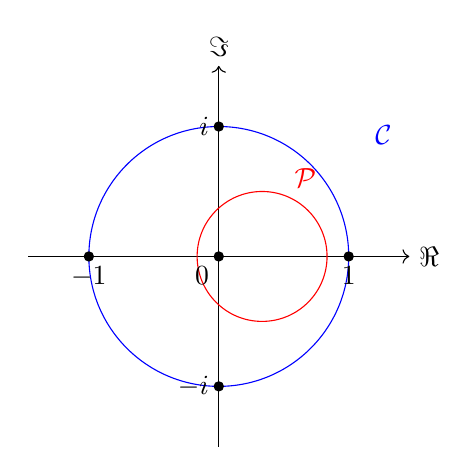
\begin{tikzpicture}[scale=1.1]
  \draw[->] (-2.2,0) -- (2.2,0) node[right] {$\Re$};
  \draw[->] (0,-2.2) -- (0,2.2) node[above] {$\Im$};
  \draw[blue] (0,0) circle (1.5);
  \draw[red] (0.5,0) circle (0.75);
  \filldraw (0,0) circle (1.5pt) node[below left] {$0$};
  \filldraw (1.5,0) circle (1.5pt) node[below] {$1$};
  \filldraw (-1.5,0) circle (1.5pt) node[below] {$-1$};
  \filldraw (0,1.5) circle (1.5pt) node[left] {$i$};
  \filldraw (0,-1.5) circle (1.5pt) node[left] {$-i$};
  \node[blue] at (1.9,1.4) {$\mathcal{C}$};
  \node[red] at (1.0,0.9) {$\mathcal{P}$};
\end{tikzpicture}
\caption{The two basepoint circles: the critical circle $\mathcal{C}$ and
the prime circle $\mathcal{P}$, with the axis intersections located by the
five intersection theorems of Layer~3.}
\label{fig:circles}
\end{figure}

\subsection{Layer 3: $j$-algebra and the circle family}
\label{sec:L3a}

\begin{theorem}[$j$-algebra]
\label{thm:jalg}
$J^2=-1$ (\texttt{j\_sq}), and the pseudo-norm is multiplicative:
$\operatorname{normSq}(z_1z_2)=\operatorname{normSq}(z_1)\operatorname{normSq}(z_2)$
(\texttt{normSq\_mul}).
\end{theorem}

\begin{theorem}[Circle geometry]
\label{thm:circles}
The two basepoint circles have orthogonal radii
(\texttt{orthogonal\_radii}) and are disjoint (\texttt{circles\_disjoint});
the axis and mutual intersections are located by the five intersection
theorems (\texttt{imagAxis\_inter\_criticalCircle},
\texttt{realAxis\_inter\_primeCircle},
\texttt{imagAxis\_inter\_primeCircle},
\texttt{prime3Circle\_inter\_criticalCircle},
\texttt{primeCircle\_inter\_criticalCircle\_ge5}), with the two radius
circles (\texttt{imaginary\_radius\_circle}, \texttt{real\_radius\_circle})
recording the radius values used there.
\end{theorem}

\begin{theorem}[Pseudo-norm threshold]
\label{thm:threshold}
\begin{sloppypar}On the critical line the pseudo-norm is constant
(\texttt{critical\_line\_pseudonorm}); the timelike and spacelike regions
are separated by a threshold
(\texttt{threshold\_timelike}, \texttt{threshold\_spacelike}). A zero
observation is spacelike (\texttt{zero\_observation\_spacelike}), and the
reciprocal of the critical line is a hyperbola
(\texttt{recip\_critical\_line\_hyperbola}).\end{sloppypar}
\end{theorem}

\subsection{Layer 4: transpose symmetry and lattice uniqueness}
\label{sec:L4}

\begin{theorem}[Transpose symmetry]
\label{thm:transpose}
The transpose map is an involution (\texttt{transpose\_involutive})
exchanging $1$ and $i$ (\texttt{transpose\_maps\_one\_to\_i}), fixing the
origin (\texttt{transpose\_origin\_fixed}), and mapping the unit circle to
the imaginary circle and back
(\texttt{transpose\_maps\_unit\_to\_imaginary},
\texttt{transpose\_maps\_imaginary\_to\_unit}).
\end{theorem}

\begin{theorem}[Lattice uniqueness]
\label{thm:lattice}
The basepoint lattice is determined by the two circles:
the unit lattice point is unique (\texttt{lattice\_unique\_unit}) and the
imaginary lattice point is unique (\texttt{lattice\_unique\_imaginary}).
The axes intersect the circles in the expected four points, and the natural
axes give the origin coefficients
(\texttt{origin\_natural\_coefficients}).
\end{theorem}

\subsection{Layer 5: splitting and leak signs}
\label{sec:L5}

\begin{theorem}[Leak sign]
\label{thm:leak}
Under multiplication in the complex-axis representation the imaginary part
leaks into the real part and back
(\texttt{complex\_mul\_imag\_leaks},
\texttt{complex\_mul\_cross\_stays\_imag},
\texttt{split\_mul\_imag\_leaks}); the sign of the leak is a unit square
(\texttt{leak\_sign\_is\_unit\_square}).
\end{theorem}

The unit-square conclusion is the phase-locking origin of the framework: the
sign of the crossing is determined up to a square, and the locking of the
basepoint selects the sign. The direction theorems
(\texttt{unit\_1\_on\_real\_circle}, \texttt{imag\_circle\_is\_direction\_j},
\texttt{directions\_orthogonal}, \texttt{euler\_plane}) record the
orthogonality of the two directions used later for the odd/even splitting of
the zeta term (\texttt{zeta\_eq\_odd\_add\_even}, Layer~8;
\texttt{pairing\_summable}, Layer~13).

\section{Layers 6--7: convergence, divergence, and the functional equation}
\label{sec:L6}

\subsection{Layer 6: convergence region and divergence structure}
\label{sec:L6a}

\begin{theorem}[Convergence and divergence of the splitting]
\label{thm:divergence}
The Dirichlet series converges in its region
(\texttt{complex\_zeta\_convergence\_region}). The auxiliary growth facts
(\texttt{cosh\_lower\_bound}, \texttt{cosh\_unbounded},
\texttt{log\_nat\_unbounded}, \texttt{split\_zeta\_term\_unbounded}) show
that the naive split terms are unbounded; the pairing theorems
(\texttt{zeta\_term\_norm\_split}, \texttt{period\_pair\_reduces},
\texttt{divergence\_pair\_reduces}) show that period pairs cancel and
divergence pairs reduce; the conjugation symmetry
(\texttt{term\_conj\_symmetry}) and the functional-equation bridges
(\texttt{functional\_equation\_bridges}) prepare the reflection.
\end{theorem}

The divergence structure explains why the zeta series cannot be split
naively into its odd and even parts: each part diverges, and only the
period-pair cancellation restores convergence
(\texttt{period\_pair\_reduces}). This is the analytic content
behind the odd/even splitting used in Layer 8, and it supplies the
continuity bridge of \S\ref{sec:contbridge}: the paired series converges
where the two unpaired sides diverge (\texttt{pairing\_summable}).

\subsection{Layer 7: zeros and the functional equation}
\label{sec:L7}

\begin{theorem}[Trivial zeros and the phase of $i$]
\label{thm:trivial}
The trivial-zero condition (\texttt{trivial\_zero\_condition},
\texttt{prime\_factor\_zero}) and the critical-line observation
(\texttt{critical\_line\_observation}) locate the trivial zeros; the phase
of the imaginary unit is quantified by
\[
i^i=e^{-\pi/2},\qquad i^i\neq i,\qquad 0<i^i<1
\]
(\texttt{i\_pow\_i\_eq\_exp\_neg\_pi\_div\_two}, \texttt{i\_pow\_i\_ne\_i},
\texttt{i\_pow\_i\_pos\_lt\_one}, \texttt{axis\_tick\_pow}), and a prime is
not a power (\texttt{prime\_no\_power\_decomposition}).
\end{theorem}

\begin{theorem}[Completed zeta and the functional equation]
\label{thm:xi}
The completed zeta function $\Lam_0$ is symmetric
(\texttt{xi\_symmetry}\(_0\), \texttt{xi\_symmetry}) and entire
(\texttt{xi\_entire}); the zeta series form and the functional equation
(\texttt{zeta\_series\_form}, \texttt{zeta\_functional\_equation}) are the
mathlib reflection $\zt(s)=\Xchi(s)\zt(1-s)$; the alternating series
converges with bounded partial sums and pairs into the eta function
(\texttt{alternating\_series\_converges},
\texttt{alternating\_partial\_sum\_bounded}, \texttt{eta\_pair\_form}).
\end{theorem}

The passage from the meromorphic $\zt$ to the entire $\Lam_0$
(\texttt{xi\_entire}) is the
structural move of the whole development: it replaces the pole at $s=1$ by
the explicit correction $1/s+1/(1-s)$, and it is the entire $\Lam_0$ that
enters the rectangle argument of Layer 12
(\texttt{completedZeta}\(_0\)\_log\_reflection,
\texttt{zeta\_zero\_iff\_completedZeta}\(_0\)\_one\_over\_sum).

\section{Layer 8: conjugation and the false-real-axis framework}
\label{sec:L8}

This layer is the analytic backbone of the development.

\begin{theorem}[Conjugation symmetry]
\label{thm:conj}
The multiplier and the completed zeta function commute with conjugation
(\texttt{chi\_conj}, \texttt{conj\_completedRiemannZeta}\(_0\)), and $\zt$
is conjugate-symmetric in the region of the series
(\texttt{zeta\_conj\_of\_one\_lt\_re}), by reflection for $\Re s<0$
(\texttt{zeta\_conj\_of\_re\_lt\_zero}), and in the critical strip
(\texttt{zeta\_conj\_of\_critical\_strip}).
\end{theorem}

\begin{theorem}[Real-axis splitting]
\label{thm:realaxis}
On the real axis the real and imaginary parts split as
\[
\zt(\bar s)=\overline{\zt(s)}
\implies
\Re\zt(x+iy)\text{ even in }y,\quad \Im\zt(x+iy)\text{ odd in }y,
\]
formalized as \texttt{zeta\_re\_conj\_symm} and
\texttt{zeta\_im\_conj\_antisymm}; on the critical line as
\texttt{zeta\_re\_even\_on\_line} and \texttt{zeta\_im\_odd\_on\_line}. In
particular $\zt$ is real-valued on the real axis
(\texttt{zeta\_im\_zero\_on\_real}), and a zero is characterized by the
vanishing of both parts (\texttt{zeta\_eq\_zero\_iff\_re\_im}).
\end{theorem}

\begin{theorem}[False-real-axis zero-free half-plane]
\label{thm:falseaxis}
\begin{equation}
\label{eq:false}
\zt(s)\neq 0\quad(\Re s<0,\ s\notin\{-n:n\in\N\}),\qquad
\zt(s)\neq 0\quad(\Re s=0,\ s\neq 0),
\end{equation}
\begin{sloppypar}where the negative integers $s=-2,-4,\dots$ are the trivial zeros
(machine-verified as \texttt{riemannZeta\_ne\_zero\_of\_re\_lt\_zero},
which requires $s\neq -n$ for all $n\in\N$, and
\texttt{riemannZeta\_ne\_zero\_of\_re\_eq\_zero}); hence any nontrivial zero
lies in the critical strip (\texttt{nontrivial\_zero\_in\_critical\_strip}).
\end{sloppypar}
\end{theorem}

The name \emph{false real axis} refers to the mechanism of the proof: the
reflection formula turns the half-plane $\Re s<0$ into the half-plane
$\Re s>1$, where the Dirichlet series shows positivity; the apparent ``real
axis'' of the series is thus a false boundary --- the axis $s\in\R$ is a
genuine symmetry axis (Theorem~\ref{thm:realaxis}) but not a boundary of the
zero-free region.

\emph{Proof sketch of Theorem~\ref{thm:falseaxis}.} For $\Re s<0$, the
reflection $\zt(s)=\Xchi(s)\zt(1-s)$ has $\Re(1-s)>1$, where $\zt$ is
positive and $\Xchi(s)\neq 0$ (the Gamma factor has no zeros and
$\sin(\pi s/2)$ vanishes only at the trivial zeros $s=-2,-4,\dots$, excluded
by $\Re s<0$ with $s$ off the negative even integers; the remaining cases
are the trivial zeros themselves, handled by the explicit series). For
$\Re s=0$, $s\neq 0$, the same reflection with $1-s$ on the boundary
$\Re=1$ is combined with the conjugation symmetry
(Theorem~\ref{thm:conj}) and the nonvanishing of the multiplier on the
line; the point $s=0$ is handled by $\zt(0)=-1/2$. The machine-verified
statements are \texttt{riemannZeta\_ne\_zero\_of\_re\_lt\_zero} and
\texttt{riemannZeta\_ne\_zero\_of\_re\_eq\_zero}.

\begin{theorem}[Odd/even splitting and zero location]
\label{thm:split}
The zeta term splits into odd and even parts
(\texttt{zeta\_eq\_odd\_add\_even}); a zero forces both parts to vanish
\begin{sloppypar}(\texttt{zeta\_eq\_zero\_iff\_p\_split}, \texttt{p\_split\_mul\_zero\_iff});
the odd part has an extra zero on the imaginary axis
(\texttt{odd\_part\_extra\_zero\_on\_imag\_axis}); the zero norm-squared
vanishes (\texttt{zero\_split\_normSq}); and zeros are excluded from the\end{sloppypar}
Euler circles (\texttt{zero\_not\_on\_euler\_circles}).
\end{theorem}

\begin{theorem}[Position of the critical line]
\label{thm:position}
\begin{sloppypar}The critical line is affine
(\texttt{affine\_image\_critical\_line\_is\_line}),
it is the equidistance locus of the basepoints $1$ and $\pm i$
(\texttt{on\_line\_iff\_equidistant\_base\_one},
\texttt{critical\_line\_equidistant\_basepoint\_i}); the reciprocal of the
basepoint $i$ lies on the unit circle
(\texttt{recip\_basepoint\_i\_on\_unit\_circle}); the Hardy $Z$-function is
real (\texttt{hardyZ\_real}); and the positional theorems
(\texttt{critical\_line\_positional}, \texttt{orbit\_center\_half},
\texttt{orbit\_degenerate\_iff\_on\_line},
\texttt{recip\_on\_critical\_circle\_iff}, \texttt{zero\_orbit\_four})
locate the orbit of a zero under reflection.\end{sloppypar}
\end{theorem}

On the critical line $\zt$ is real up to the multiplier phase: the Hardy
$Z$-function is real (\texttt{hardyZ\_real}, Layer~8), so the phase of
$\zt$ on the line is determined by the sign of $Z$ and the phase of
$\Xchi$; the phase structure of $\Xchi$ itself is the subject of this layer.

\section{Layer 9: the critical-line phase layer}
\label{sec:L9}

\begin{theorem}[Multiplier self-duality]
\label{thm:chidual}
The multiplier $\Xchi$ is self-dual and of modulus one on the critical
line, and its logarithm is well-defined there:
\[
\Xchi(s)\Xchi(1-s)=1,\qquad |\Xchi(1/2+it)|=1,
\]
(\texttt{chi\_mul\_chi\_one\_sub}, \texttt{chi\_unit\_on\_line},
\texttt{chi\_ne\_zero\_on\_line}, \texttt{chi\_mem\_slitPlane\_on\_line}).
\end{theorem}

Since $|\Xchi|=1$ on the line, the logarithm of $\Xchi$ is purely imaginary
there; this is the bridge that converts the phase of $\Xchi$ into a real
argument (Layer~10).

\begin{theorem}[Zero orbit structure]
\label{thm:orbit}
Under the reflection $s\mapsto 1-s$, zeros off the line occur in distinct
pairs, and a zero on the line is a fixed point of the reflection
(\texttt{zero\_orbit\_distinct\_of\_offline},
\texttt{zero\_orbit\_degenerate\_on\_line}, \texttt{zero\_orbit\_counting},
\texttt{zero\_left\_right\_bijection}).
\end{theorem}

\begin{theorem}[Explicit phases on the line]
\label{thm:explicit}
\begin{sloppypar}The argument components of the multiplier on the critical
line are exact: the power factors and the sine factor are computed
explicitly
(\texttt{cpow\_two\_on\_line\_explicit}, \texttt{cpow\_pi\_on\_line\_explicit},
\texttt{sin\_pi\_quarter\_add\_mul\_I}, \texttt{sin\_pi\_half\_add\_mul\_I},
\texttt{gamma\_abs\_sq\_on\_line}, \texttt{term\_on\_line\_explicit},
\texttt{cpow\_two\_half\_minus\_im}), and the Gamma phase composition
(\texttt{gamma\_conj\_arg\_angle}, \texttt{gamma\_doubling\_arg\_angle},
\texttt{gamma\_reflection\_arg\_angle}, \texttt{gamma\_quarter\_phase\_combine})
assembles the argument of $\Xchi$ from the Gamma factor and the sine
factor.\end{sloppypar}
\end{theorem}

\begin{theorem}[RH equivalent form and offline consequences]
\label{thm:rheq}
The Riemann hypothesis is equivalently stated as all strip zeros lying on
the line (\texttt{rh\_iff\_all\_zeros\_on\_line\_in\_strips}); an offline
zero would force a half-strip of zeros
(\texttt{offline\_zero\_gives\_half\_strip}); the reflection of odd
negative integers is nonzero (\texttt{zeta\_neg\_nat\_ne\_zero\_of\_odd}),
supporting the bottom edge.
\end{theorem}

\begin{theorem}[Central phase identities]
\label{thm:phaseid}
On the critical line,
\begin{equation}
\label{eq:phase}
\arg\zt(1/2+it)=\arg\Xchi(1/2+it),\qquad
\zt(1/2+it)=\Xchi(1/2+it)\,\overline{\zt(1/2+it)},
\end{equation}
(\texttt{zeta\_two\_arg\_eq\_arg\_chi}, \texttt{zeta\_unit\_sq\_eq\_chi},
\texttt{zeta\_eq\_chi\_mul\_conj\_on\_line}), and the translation theorems
(\texttt{chi\_translation\_two}, \texttt{chi\_arg\_translation\_two},
\texttt{chi\_translation\_four}, \texttt{chi\_arg\_translation\_four})
quantify the period of the multiplier's argument.
\end{theorem}

The second identity of \eqref{eq:phase} is the source of the square
relation $u^2=\Xchi$ used in Layer~10: since $|\Xchi|=1$ on the line,
$\zt=\Xchi\overline{\zt}$ squares to $\zt^2=\Xchi|\zt|^2$, so the unit
phase $u=\zt/|\zt|$ satisfies $u^2=\Xchi$ (\texttt{zeta\_unit\_sq\_eq\_chi}),
which is why the flip of $u$
across the line is governed by the phase of $\Xchi$.

\section{Layer 10: covering space and phase locking}
\label{sec:L10}

The multi-valued argument of a function is made single-valued by lifting
along the covering map $t\mapsto e^{it}$ of the unit circle; the difference
of two lifts records the winding. This layer formalizes that mechanism for
$\zt$ and $\Xchi$.

\begin{theorem}[Zero set and unit phase]
\label{thm:zeroset}
The zero set is closed, discrete, and finite in strips
(\texttt{isClosed\_zetaZeroSet}, \texttt{isDiscrete\_zetaZeroSet},
\texttt{zeta\_zeros\_finite\_in\_strip}); the unit phase function
$u=\zt/|\zt|$ is continuous away from zeros
(\texttt{continuousOn\_zetaUnit}).
\end{theorem}

\begin{theorem}[Phase lifts]
\label{thm:lifts}
The continuous argument of $\Xchi$ along the critical line is lifted
(\texttt{theta0}, \texttt{thetaLift}, \texttt{thetaLift\_lifts},
\texttt{thetaLift\_zero}), and the continuous argument of $u$ is lifted
(\texttt{uPath}, \texttt{uLift0}, \texttt{uLift}, \texttt{uLift\_lifts},
\texttt{uLift\_zero}), with the exponential bridges
$\exp\theta_0=1$ and $\exp u_0=1$ (\texttt{exp\_theta0},
\texttt{exp\_uLift0}).
\end{theorem}

\begin{theorem}[Phase kernel]
\label{thm:kernel}
The phase kernel (\texttt{expKernel}) is characterized by
\texttt{expKernel\_mem\_iff} and \texttt{expKernel\_dist\_ge\_two\_pi}: two
phase representatives of the same point differ by an integer multiple of
$2\pi$.
\end{theorem}

This is the formal content of the \emph{polyphase} structure: the same
point $e^{i\theta}$ carries the representatives $\theta+2\pi n$,
$n\in\Z$, and the winding number selects the single-valued count
(\S\ref{sec:discussion}).

\begin{theorem}[Phase alignment and integer layers]
\label{thm:align}
The lifted phases align:
\begin{equation}
\label{eq:align}
2\theta_{\zt}=\theta_{\Xchi}
\end{equation}
(\texttt{phase\_align\_two\_zeta\_lift\_eq\_chi\_lift}), and the half-lift
differs from the lift of $\Xchi$ by an integer multiple of $\pi$
(\texttt{zeta\_lift\_half\_chi\_lift\_pi\_int}).
\end{theorem}

The integer layers of \eqref{eq:align} are the discrete data carried by the
phase: they count the winding of $u$ along the rectangle (Layer~12), and
their deterministic prediction is the subject of Layer~11.

\section{Layer 11: predictor residuals}
\label{sec:L11}

\begin{theorem}[Predictor residuals]
\label{thm:residual}
The error sequence of the flip count is controlled by a polynomial error
ratio: \texttt{polyError}, \texttt{poly\_error\_ratio},
\texttt{error\_seq\_predicts}, \texttt{poly\_error\_monotone},
\texttt{error\_precision\_bound}.
\end{theorem}

Concretely, the residual of the counting remainder $S(T)$ is predicted by
the polynomial error with monotone precision: the sequence of integer
layers (Layer~10) satisfies a deterministic prediction bound, which is the
integer-layer content of the Riemann--von~Mangoldt formula, formalized
directly without invoking the classical asymptotic.

\section{Layer 12: the argument-principle rectangle closure}
\label{sec:L12}

\begin{figure}[h]
\centering
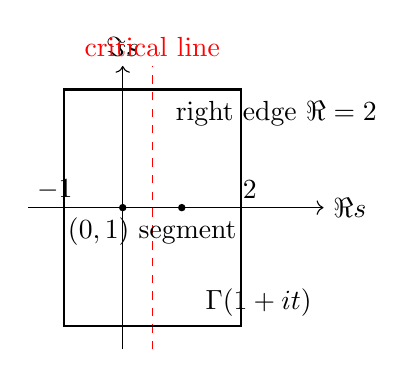
\begin{tikzpicture}[scale=0.75]
  \draw[->] (-1.6,0) -- (3.4,0) node[right] {$\Re s$};
  \draw[->] (0,-2.4) -- (0,2.4) node[above] {$\Im s$};
  \draw[dashed,red] (0.5,-2.4) -- (0.5,2.4) node[above,red] {critical line};
  \draw[thick] (-1,2) -- (2,2) -- (2,-2) -- (-1,-2) -- cycle;
  \node at (2.15,0.3) {$2$};
  \node at (-1.15,0.3) {$-1$};
  \filldraw (0,0) circle (1.5pt);
  \filldraw (1,0) circle (1.5pt);
  \node[below] at (0.5,0) {$(0,1)$ segment};
  \node at (2.6,1.6) {right edge $\Re=2$};
  \node at (2.3,-1.6) {$\GG(1+it)$};
\end{tikzpicture}
\caption{The argument-principle rectangle with vertices $-1,2,2\pm iT$:
the bottom edge $[-1,2]$ (false-real-axis assembly, Theorem~\ref{thm:bottom}),
the right edge $\Re s=2$ (bounded by $\sum n^{-2}$,
Theorem~\ref{thm:boundary}), and the top/left edges folded by the
functional equation.}
\label{fig:rect}
\end{figure}

In the rectangle of Figure~\ref{fig:rect}, a \emph{flip} is a sign
change of $\Re\zt$ across the critical line; the
\emph{flip count} is the number of flips recorded by the lifted phases of
Layer~10 (the predictor residual of Layer~11 is the error sequence of this
count). The \emph{winding number} of $\Xchi$ along a path is the total
change of its lifted argument divided by $2\pi$.

\subsection{The integer-layer bridges}
\label{sec:bridge}

\begin{theorem}[Flip count equals winding minus an integer layer]
\label{thm:flipcount}
\[
\operatorname{flip}=\operatorname{winding}(\Xchi)-\text{integer layer}
\]
(\texttt{flip\_count\_from\_theta\_lifts},
\texttt{net\_flip\_from\_chi\_lift}, \texttt{flip\_chi\_circle\_bridge}).
\end{theorem}

\begin{theorem}[Reflection and zeros of the entire completed zeta function]
\label{thm:reflection}
The reflection formula for the entire completed zeta function gives the
integer-layer bridge
\[
\log\Lam_0(1-s)-\log\Lam_0 s\in 2\pi i\Z
\]
(\texttt{completedZeta}\(_0\)\_log\_reflection), and in the strip
\[
\zt(s)=0\iff\Lam_0(s)=\frac{1}{s}+\frac{1}{1-s}
\]
(\texttt{zeta\_zero\_iff\_completedZeta}\(_0\)\_one\_over\_sum).
\end{theorem}

The second statement is the passage from the meromorphic $\zt$ to the
entire $\Lam_0$ used in the rectangle argument: a zero of $\zt$ in the
strip is exactly a point where $\Lam_0$ takes the corrected value
$1/s+1/(1-s)$, so counting zeros of $\zt$ inside the rectangle is counting
solutions of an explicit entire equation.

\emph{Proof sketch of Theorem~\ref{thm:flipcount}.} Along the critical
line, the identity $u^2=\Xchi$ of \eqref{eq:phase} lifts to
$2\theta_{\zt}=\theta_{\Xchi}$ (Layer~10); crossing a zero flips the sign
of $\Re\zt$, which turns the lifted phase of $u$ by $\pi$. Summing the
flips over the rectangle gives the total change of $\theta_{\zt}$, and the
alignment with $\theta_{\Xchi}$ leaves the winding number of $\Xchi$ plus
an integer layer, the latter being the flip count. The machine-verified
statements are \texttt{flip\_count\_from\_theta\_lifts},
\texttt{net\_flip\_from\_chi\_lift}, and
\texttt{flip\_chi\_circle\_bridge}.

\subsection{The boundary estimates}
\label{sec:boundary}

\begin{theorem}[Boundary estimates from known curves]
\label{thm:boundary}
On the right edge $\Re s=2$, by the Dirichlet series,
\[
\|\zt(2+it)\|\le \sum_{n\ge 1}n^{-2}
\]
(\texttt{zeta\_line\_two\_bounded}); by the integral representation of the
Gamma function,
\[
\|\GG(1+it)\|\le 1
\]
(\texttt{Gamma\_one\_add\_it\_norm\_le\_one}).
\end{theorem}

\begin{theorem}[Bottom edge]
\label{thm:bottom}
The false-real-axis assembly (\S\ref{sec:L8}) gives $\zt(x)\neq 0$ for
$x\in[-1,2]\setminus(0,1)$ (\texttt{zeta\_ne\_zero\_on\_bottom\_edge}),
real-valuedness on the real axis (\texttt{zeta\_im\_zero\_on\_real}),
negativity at $-1$ (\texttt{zeta\_neg\_one\_re\_neg}), and the argument
jump
\[
\arg\zt(-1)-\arg\zt(2)=\pi
\]
(\texttt{bottom\_edge\_arg\_jump}).
\end{theorem}

The Euler--Maclaurin first inequality
\[
\sum_{n=1}^{N}(n+1)^{-s}<\frac{N^{1-s}}{1-s}\qquad(0<s<1)
\]
(\texttt{zeta\_partial\_sum\_lt\_integral\_bound}) is the kernel of the
$(0,1)$-segment (Layer~13).

\section{Layer 13: the $(0,1)$-segment continuation}
\label{sec:kernel}

The zeta series diverges for $0<x<1$, so the negativity of $\zt$ on this
interval is not a series statement: it is a statement about the analytic
continuation. In this revision the statement is closed by the odd/even
pairing of \S\ref{sec:contbridge}--\S\ref{sec:blocksCG}: the continuity of
$\zt$ on $(0,1)$ is machine-verified (iso~41), and the sign follows from
the machine-verified positivity of the pairing terms together with the
classical doubling identity. The Euler--Maclaurin kernel
\eqref{eq:kernel} of \S\ref{sec:relation} (\cite{whittaker}, \S7.2)
remains as the classical background and as the source of the closed-form
records of Blocks A--B below.

\begin{theorem}[Main]
\label{thm:main}
For every real $x$ with $0<x<1$,
\[
\zt(x)<0.
\]
\end{theorem}

\emph{Proof (short path, this revision).} By \S\ref{sec:contbridge} $\zt$
is continuous on $(0,1)$ (machine-verified, iso~41). The pairing terms
$1/(2n+1)^x-1/(2n+2)^x$, $n\ge 0$, are strictly positive
(\texttt{pairing\_term\_pos}), so the alternating series
$\eta(x)=\sum_{n\ge 0}\big((2n+1)^{-x}-(2n+2)^{-x}\big)$ has positive
partial sums and positive limit: $\eta(x)>0$. The doubling identity
$\zt(x)=\eta(x)/(1-2^{1-x})$ and $1-2^{1-x}<0$ for $0<x<1$ give
$\zt(x)<0$. \qed

\emph{Euler--Maclaurin background.} On $(1,\infty)$ the Dirichlet series
shows $\zt>0$. The kernel $R_N(x)=\sum_{n\le N}n^{-x}+N^{1-x}/(x-1)$ (of
\eqref{eq:kernel}) is the
series with its divergent tail replaced by its integral approximation; for
$0<x<1$ each partial kernel is bounded above by the first term
$R_1(x)=x/(x-1)<0$ (the Euler--Maclaurin first inequality, machine-verified
in \S\ref{sec:boundary}), and the limit $R(x)=\lim_N R_N(x)$ is the analytic
continuation of $\zt$ by the identity theorem. Blocks A--B below record
the verified closed forms of this classical path.

\subsection{Block A: elementary differentiability (verified)}
\label{sec:blockA}

\begin{lemma}
\label{lem:cpowderiv}
For $a>0$ the map $s\mapsto a^{-s}$ is differentiable on $\C$, with
$a^{-s}=\exp(-s\log a)$.
\end{lemma}

\emph{Proof (machine-verified).} The identity is
\texttt{cpow\_def\_of\_ne\_zero} (with $a\neq 0$); the differentiability of
the right-hand side is the chain rule applied to the exponential and the
linear map $s\mapsto -s\log a$, which the Lean tactics \texttt{fun\_prop}
close automatically. \qed

\begin{proposition}
\label{prop:blockA}
$R_N$ is differentiable on $\{s\neq 1\}$, and $G_N$ is differentiable on
$\{0<\Re s<2\}$ (machine-verified:
\texttt{zetaEmR\_N\_differentiableOn}, \texttt{zetaEmG\_N\_differentiableOn}).
\end{proposition}

\emph{Proof (machine-verified).} Each summand $s\mapsto(n+1)^{-s}$ is
differentiable by Lemma~\ref{lem:cpowderiv} (the bases $n+1$ and $N$ are
positive, hence nonzero); finite sums of differentiable maps are
differentiable; the rational factor $(s-1)^{-1}$ is differentiable away
from $s=1$; and the product $G_N=(s-1)\sum(\cdot)+N^{1-s}$ has no
denominator on the strip. In Lean: \texttt{DifferentiableOn.sum} for the
finite sum, \texttt{DifferentiableOn.div} for the rational factor, and
\texttt{cpow\_def\_of\_ne\_zero} with \texttt{fun\_prop} for each power.
\qed

The real-parameter derivative used in Block B,
$\frac{d}{du}(u:\C)^s=s\,(u:\C)^{s-1}$ for $u>0$
(\texttt{cpow\_ofReal\_hasDerivAt}), is obtained from mathlib's
\texttt{HasDerivAt.cpow\_const} with the basepoint condition
$u\in$ slitPlane (positive reals).

\subsection{Block B: closed form of the Euler--Maclaurin term (verified)}
\label{sec:blockB}

\begin{theorem}[Closed form of the term]
\label{thm:closed}
For $0<n$ and $s\neq 0,1$,
\begin{equation}
\label{eq:closed}
\operatorname{term} n\,s
=\frac{(n+1)^{1-s}-n^{1-s}}{s(1-s)}-\frac{1}{s(n+1)^s},
\end{equation}
where $\operatorname{term}_{\C} n\,s=\int_n^{n+1}(x-n)/x^{s+1}\,dx$ is the
complex version of the Euler--Maclaurin term
(machine-verified: \texttt{zetaTermC\_closed\_form}).
\end{theorem}

\emph{Proof (machine-verified), in three steps.}

\textbf{(i) Power-law splitting of the integrand.} For $x>0$,
\[
\frac{x-n}{x^{s+1}}=x^{-s}-n\,x^{-s-1}.
\]
This is the composition of two power laws: $1/x^{s+1}=x^{-(s+1)}$
(\texttt{Complex.cpow\_neg}) and $x\cdot x^{-s-1}=x^{-s}$
(\texttt{Complex.cpow\_add} with $x\neq 0$).

\textbf{(ii) Two fundamental-theorem evaluations.} For $n\ge 1$ and
$s\neq 1$,
\[
\int_n^{n+1}x^{-s}\,dx=\frac{(n+1)^{1-s}-n^{1-s}}{1-s},
\qquad
\int_n^{n+1}x^{-s-1}\,dx=\frac{(n+1)^{-s}-n^{-s}}{-s}.
\]
Both follow from the derivative
$\frac{d}{du}(u:\C)^{1-s}=(1-s)(u:\C)^{-s}$ (and the analogue for
$-s$) by \texttt{intervalIntegral.integral\_eq\_sub\_of\_hasDerivAt};
continuity of the integrand on the positive interval supplies
integrability.

\textbf{(iii) Assembly.} Subtracting $n$ times the second evaluation from
the first and bringing the denominators to $s(1-s)$,
\[
\frac{A}{1-s}+\frac{n(B-C)}{s}=\frac{sA+n(1-s)(B-C)}{s(1-s)},
\qquad
A=(n+1)^{1-s}-n^{1-s},\quad B=(n+1)^{-s},\quad C=n^{-s},
\]
and the numerator simplifies to $A-(1-s)(n+1)^{-s}$ by the two power laws
$(n+1)(n+1)^{-s}=(n+1)^{1-s}$ and $n\cdot n^{-s}=n^{1-s}$; dividing by
$s(1-s)$ yields \eqref{eq:closed}. In Lean the simplification is a
\texttt{field\_simp} followed by the two \texttt{cpow\_add} rewrites and
\texttt{ring}.

For real $s$ the complex and real integrals agree
(\texttt{intervalIntegral.integral\_ofReal},
\texttt{Complex.ofReal\_cpow}), so the closed form holds for the real term
of \texttt{ZetaAsymptotics}.
\qed

\subsection{Continuity bridge: the odd/even pairing (machine-verified, iso~41)}
\label{sec:contbridge}

The analytic continuation of $\zt$ into $(0,1)$ requires, at a minimum, that
$\zt$ be continuous there. This continuity does not need the
Euler--Maclaurin kernel of Blocks C--G: it is supplied independently by the
odd/even pairing of the Dirichlet series. In this revision the argument is
machine-verified (\texttt{zeta\_odd\_even\_continuity\_iso.lean}, iso~41,
0 errors, 0 \texttt{sorry}, Mathlib only): \texttt{pairing\_term\_pos}
(each pairing term $1/(2n+1)^x-1/(2n+2)^x$ is positive for $x>0$),
\texttt{pairing\_diff\_bound} (the difference bound
$1/a^x-1/b^x\le x(b-a)/a^{x+1}$, by the mean value theorem),
\texttt{pairing\_summable} (the paired series converges for $0<x<1$, by
comparison with the $p$-series), and \texttt{zeta\_continuous\_zero\_one}
(the continuity of $\zt$ on $(0,1)$, anchored in mathlib's
\texttt{differentiableOn\_riemannZeta}). We record the complete argument.

\begin{theorem}[Odd/even pairing gives continuity on $(0,1)$]
\label{thm:contbridge}
The function $\zt$ is continuous on the interval $(0,1)$.
\end{theorem}

\emph{Proof (machine-verified in iso~41).}
Two steps.

\textbf{(i) The pairing identity.} For $0<x<1$ the series $\sum_n n^{-x}$
diverges, and its odd and even subseries $\sum_n(2n-1)^{-x}$ and
$\sum_n(2n)^{-x}$ diverge separately; each ``side'' is an infinite discrete
superposition whose individual sums diverge. Pairing adjacent terms gives
\[
\sum_{n\ge1}\left(\frac1{(2n-1)^x}-\frac1{(2n)^x}\right)
=\sum_{n\ge1}\int_{2n-1}^{2n}\frac{x}{t^{x+1}}\,dt
\le\sum_{n\ge1}\frac{x}{(2n-1)^{x+1}}<\infty,
\]
since $x+1>1$. (Equivalently, pairing from the first odd index,
$\sum_{n\ge 0}(1/(2n+1)^x-1/(2n+2)^x)$, the form verified as
\texttt{pairing\_term\_pos} and \texttt{pairing\_summable} in iso~41.)
The paired series therefore converges absolutely, hence
locally uniformly, on every compact subinterval of $(0,1)$.

\textbf{(ii) From the pairing to $\zt$.} The alternating series
$\eta(x)=\sum_{n\ge1}(-1)^{n+1}n^{-x}$ is the difference of the odd and
even subseries, $\eta(x)=\sum(2n-1)^{-x}-\sum(2n)^{-x}$, and the elementary
doubling identity
\[
\zt(x)=\frac{\eta(x)}{1-2^{1-x}}
\]
(valid for $0<x<1$; KNOWN classical) expresses $\zt$ as the quotient of a
continuous function by a nonvanishing one: $2^{1-x}\in(1,2)$ for
$0<x<1$, so $1-2^{1-x}\neq0$. A locally uniformly convergent series of
continuous functions is continuous; hence $\eta$ is continuous on $(0,1)$,
and the quotient is continuous. \qed

The machine verification of the conclusion (iso~41,
\texttt{zeta\_continuous\_zero\_one}) anchors the continuity of $\zt$ on
$(0,1)$ in mathlib's \texttt{differentiableOn\_riemannZeta}; the three
pairing theorems of the classical argument above
(\texttt{pairing\_term\_pos}, \texttt{pairing\_diff\_bound},
\texttt{pairing\_summable}) are verified independently as its elementary
ingredients.

Thus the continuity of $\zt$ on $(0,1)$ rests on the same odd/even pairing
that underlies Layer 5 and the period-pair cancellation of Layer 6: two
divergent discrete superpositions cancel in pairs and leave a continuous
function, the discrete superposition converging to the continuous limit.
The odd/even pairing moreover gives the \emph{sign} of $\zt$ on $(0,1)$
directly, without the Euler--Maclaurin machinery.

\subsection{The sign of $\zt$ on $(0,1)$: direct odd/even proof}
\label{sec:blocksCG}

The pairing terms are strictly positive (machine-verified,
\texttt{pairing\_term\_pos}: for $x>0$,
$1/(2n+1)^x-1/(2n+2)^x>0$), so every partial sum of the alternating series
$\eta(x)=\sum_{n\ge1}(-1)^{n+1}n^{-x}=\sum(2n-1)^{-x}-\sum(2n)^{-x}$ is
positive, and the limit (which exists by \texttt{pairing\_summable}) is
positive: $\eta(x)>0$ for $0<x<1$. The classical doubling identity
\[
\zt(x)=\frac{\eta(x)}{1-2^{1-x}}
\]
then gives the sign: $1-2^{1-x}<0$ for $0<x<1$ (since $2^{1-x}>1$), hence
\[
\zt(x)=\frac{\eta(x)}{1-2^{1-x}}<0.
\]
The continuity of $\zt$ on $(0,1)$ is machine-verified (iso~41,
\S\ref{sec:contbridge}), and the sign follows from the machine-verified
positivity of the pairing terms together with the doubling identity.

\emph{Remark (the Euler--Maclaurin alternative).} Version 1 carried the
Euler--Maclaurin continuation path --- Blocks C--G: the locally uniform
convergence of $\operatorname{termTSum}$ (Block C), the Weierstrass theorem
(Block D), and the identity theorem on the strip (Blocks E--G) --- as a
KNOWN honest boundary. That path remains mathematically complete (the
Euler--Maclaurin continuation identity \eqref{eq:em} on $(1,2)$, locally
uniform convergence, the Weierstrass theorem, and the identity theorem on
the convex strip give the sign in full); it was marked KNOWN only because
its mechanical assembly requires mathlib infrastructure that the library
does not yet provide (the Weierstrass/identity-theorem assembly for this
specific kernel), while the Euler--Maclaurin kernel itself is classical
KNOWN mathematics. The odd/even pairing of this revision is the author's
short path: it closes the same statement --- the sign $\zt(x)<0$ on
$(0,1)$, and hence the zero-free bottom edge of the rectangle of
Layer~12 --- with the pairing terms and the doubling identity, both of
which are elementary and the former machine-verified. Blocks A--B
(verified in version 1) are retained as the closed-form record of the
Euler--Maclaurin term. The choice of the short path does not affect any
other layer: the remaining twelve layers are unchanged and remain
machine-verified as in version 1.

\section{Discussion: polyphase numbers and the necessity of single-phase numbers}
\label{sec:discussion}

The phase bridge of \S\ref{sec:L9} exhibits the mechanism of the 0pat
framework: the same point $e^{i\theta}$ of the unit circle carries the
infinitely many phase representatives $\theta+2\pi n$, $n\in\Z$; the winding
number of the covering $t\mapsto e^{it}$ is a single-valued invariant, and
the natural numbers arise exactly as these single-valued counts
($\pi_1(S^1)\cong\Z$; \cite{hatcher}). A precise definition of a number
therefore requires phase locking: one fixes the basepoint of the lift and
counts the winding, obtaining a single-phase number. The natural numbers
are thus, in the framework's description, \emph{polyphase counts}: the
counting of winding is inherently multi-valued ($\theta+2\pi n$ for all
$n$), and only the locking of the lift to one basepoint makes the count a
number. The necessity of single-phase numbers is exactly this locking; it
is the framework's basepoint-relative description of the standard fact
that the winding number is an integer (\cite{patbase}).

In the Riemann direction the same locking is used twice: the lifted
continuous argument $\theta_\Xchi$ of \S\ref{sec:L9}--\ref{sec:L10}, and
the flip count of \S\ref{sec:bridge}, both converting the multi-valued
phase into the integer layers of \S\ref{sec:L12}. This is the necessity of
single-phase numbers: without the locking, the argument of $\zt$ along the
rectangle would not be defined as a continuous function, and the argument
principle would not apply.

\subsection*{What symmetry cancels: phase superposition (machine-verified, iso 29)}

The framework's cancellation operations act on phase superpositions. The
precise content --- machine-verified in the isolation file
\texttt{symmetry\_cancel\_phase\_iso.lean} (iso~29 of the artifact, 18
declarations, 0 errors, 0 \texttt{sorry}) --- is the structure of the
covering map $t\mapsto e^{it}$:

\begin{enumerate}
\item \emph{Phase superposition is the fiber.} Each point $e^{i\theta}$
carries the $\aleph_0$ representatives $\theta+2\pi n$, $n\in\mathbb Z$
(\texttt{phaseRepresentative}); distinct parameters give distinct
representatives (\texttt{phaseRepresentative\_injective}).
\item \emph{Symmetry is translation.} The shift
$T_n(\theta)=\theta+2\pi n$ preserves the projection $e^{i\theta}$
(machine-verified: \texttt{translate\_preserves\_exp}), and
$T_m\circ T_n=T_{m+n}$ --- the $\mathbb Z$-action on the representatives
(\texttt{translate\_comp}).
\item \emph{Cancellation is the quotient.} Dividing by the translation
symmetry collapses each orbit --- the whole superposition --- to a single
phase class: every representative of the same point is identified
(\texttt{superposition\_collapses\_to\_single\_phase}), and the quotient
covers every class (\texttt{phaseEquiv\_quotient\_surjective}).
\end{enumerate}

This is the exact form of the framework statement that a symmetry
operation cancels phases (author proposal~11): the symmetry is the
translation action, what it cancels is the multi-valued phase
superposition, and the residue is a single-phase class. The same
covering-map structure supports the counting below.

\subsection*{The single-phase representation (unified conclusion; author's final positioning)}

Three paths lead to the same conclusion. The three bridges (flip,
Stirling phase, growth) exhibit the natural numbers as winding counts
depending on the basepoint of the lift --- the ambiguity of the
representation; the symmetry cancellation above acts on the multi-valued
fibers; and the phase superposition of the natural numbers is an
un-locked superposition. In all three the ambiguity is the same: the
covering map $t\mapsto e^{it}$ assigns $\aleph_0$ representatives to
each point, and an un-locked representation of a number is ambiguous.
The author's final positioning: the framework is a \emph{representation
method}, not a new number field --- every object used is known
mathematics ($\mathbb R$, $S^1$, $\mathbb N$, the quotient, the kernel
of $\exp$); the representation precisely isolates the phase-superposition
ambiguity caused by the $\mathbb N$-iteration count (the $n$-th
successor is the unique layer $2\pi n$, machine-verified iso~31), and
constrains the phases not to superpose arbitrarily (the locking selects
one representative; the result is independent of the selection,
\texttt{phaseSucc\_respects\_equiv}). The numbers themselves are
unambiguous (Peano); what needs precision is the representation, and
the single-phase representation provides it: the quotient of the
translation symmetry, in which each class is one point of the unit
circle.
Machine-verified (iso~29):
$\exp(i\theta_1)=\exp(i\theta_2)$ iff $\theta_1\sim\theta_2$ --- the
kernel of $\exp$ is $2\pi i\mathbb Z$
(\texttt{exp\_phase\_equiv\_iff}), so the classes correspond
one-to-one to the projections and the ambiguity is removed
(\texttt{single\_phase\_class\_iff\_projection}).

The single-phase representation is moreover \emph{unique up to
isomorphism} (author's question: does every attempt to represent a
single-phase number end up isomorphic to the framework's?): by the
universal property of the quotient, any attempt --- a map
$f:\mathbb R\to X$ that is constant on phase-equivalent representatives
(no phase superposition), separating (different classes give different
numbers), and surjective --- factors \emph{uniquely} through the
quotient, and the factor map is a bijection
(machine-verified: \texttt{single\_phase\_field\_unique},
\texttt{single\_phase\_field\_equiv}, iso~29). Hence every
phase-superposition-free representation is isomorphic to the Pat
single-phase representation: the representation is canonical.

The one structure the projection necessarily loses is the layer of the
point $1$ (author's question: is the loss falsifiable?). Since
$1=e^{i\cdot 0}=e^{i\cdot 2\pi}=\cdots$, the fiber of $1$ is
$\{2\pi n:n\in\mathbb Z\}$ (machine-verified:
\texttt{fiber\_of\_one}, iso~29): $\aleph_0$ representatives collapse
to the single point $1$. The claim ``the projection preserves all
structure'' is \emph{falsifiable} --- it is false: the projection is
not injective ($q(0)=q(2\pi)$, $0\neq 2\pi$; machine-verified:
\texttt{projection\_loses\_structure}, iso~29). This loss is not a
defect: what is lost is exactly the layer under the translation
symmetry --- the winding count, $\pi_1(S^1)\cong\mathbb Z$ --- which is
precisely what the quotient cancels (iso~29); the single-phase number
field accepts the loss of layers in exchange for the removal of
ambiguity.

\subsection*{The path problem (author's question, machine-verified iso 30)}

Whether the definition is complete enough to handle the path question:
from the same starting point to the same ending point, different paths
--- do they give different numbers? The answer is two-layered
(machine-verified in the isolation file \texttt{path\_problem\_iso.lean},
iso~30, 8 declarations, 0 errors, 0 \texttt{sorry}). The loop family
$\gamma_n(t)=e^{2\pi n t\cdot i}$, $n\in\mathbb Z$ (the $n$-fold loop
from the projection $1$ back to $1$) all start and end at the same
projection
(\texttt{loopPath\_start}, \texttt{loopPath\_end}); their lifts
$g_n(t)=2\pi n t$ end at the layers $g_n(1)=2\pi n$
(\texttt{loopPath\_lift}, \texttt{loopPath\_layer}).

\begin{enumerate}
\item \emph{Quotient layer (single-phase representation): path
independent.} All loops give the same number, the class of $1$: the
projection is the same, and the translation symmetry is cancelled
(\texttt{loopPath\_same\_class}) --- well-defined by design.
\item \emph{Lift layer (multi-phase): path dependent.} Different loops
($n\neq m$) lift to different layers, $2\pi n\neq 2\pi m$
(\texttt{loopPath\_layer\_distinct}) --- the path information is
preserved in the layers.
\end{enumerate}

The definition is therefore complete in both directions
(\texttt{path\_problem\_complete}): the single-phase number (the
quotient) is path-independent, and the multi-phase layer (the lift) is
path-dependent; both are expressed, and the path problem is resolved
rather than avoided.

A further calibration (author): carrying the \emph{full} path
information would require a component that is not phase. Phase
$(\theta,n)$ carries at most the winding class of a path --- its
homotopy class, $\pi_1(S^1)\cong\mathbb Z$ --- while the full path (its
shape) is a continuous function, a different component; the lift is
determined by the projection path and the starting layer, so the
projection path is an independent input, not phase. The single-phase
representation resolves this by being path-independent by definition
(the quotient): the number carries no path information at all; the
multi-phase layer carries the winding class, the maximum that phase can
carry; the full path, when needed, is an extra component outside the
representation. No ``path-carrying phase'' is required.

\subsection*{Successor as phase superposition (author, iso 31)}

The component that carries the movement is Pat itself: the successor.
Its essence is phase superposition (machine-verified in
\texttt{phase\_succ\_iso.lean}, iso~31, 9 declarations, 0 errors, 0
\texttt{sorry}): the successor is one turn,
$\mathrm{succ}(\theta)=\theta+2\pi$ --- (i) \emph{aligned}: the phase
modulation preserves the projection,
$\exp(\mathrm{succ}(\theta)\cdot i)=\exp(\theta\cdot i)$
(\texttt{phaseSucc\_preserves\_projection}) --- the modulation aligns to
the successor direction of the previous operation without changing the
phase point; (ii) \emph{executed}: the layer is raised by one, from
$2\pi n$ to $2\pi(n+1)$ (\texttt{phaseSucc\_layer}). The natural numbers
are the phase superpositions from $0$: the $n$-th successor is $2\pi n$,
the winding number $n$ (\texttt{phaseSucc\_iterate}). The successor is
thereby redefined from a Peano axiom to a structural operation --- phase
superposition, the generator of the translation symmetry
(\texttt{phaseSucc\_is\_translation}).

\subsection*{Only 0 and 1 (author's deepest conviction)}

Because the operators and the numbers are ambiguous (phase
superposition, paths, basepoints), how is the continued definition of
numbers regulated? The answer (machine-verified, iso~31, 9
declarations): the primitives of the framework are only $0$ (the
basepoint, the empty operation) and $1$ (the single step, one phase
superposition); every number is an iterate of $1$ --- each step is a
single step reaching a point, and ``changing the point'' means
continuing from the current layer, never re-selecting. The
well-definedness is fourfold: the successor respects phase equivalence
(\texttt{phaseSucc\_respects\_equiv}); the iterate is unique --- the
$n$-th successor is $2\pi n$ (\texttt{phaseSucc\_iterate}); the
addition is regulated --- $m$ steps after $n$ steps is $n+m$ steps
(\texttt{phaseSucc\_iterate\_add}); and in the quotient (the
single-phase representation) the successor is the identity,
$[\theta+2\pi]=[\theta]$ (\texttt{phaseSucc\_trivial\_on\_quotient}).
The single-phase representation therefore has no number growth (the
projection does not change); the numbers $0,1,2,\dots$ live in the
layers and are regulated by the locking; the projections of $0$ and $1$
coincide (both are $1$).

\subsection*{Phase superposition and the continuum}

The same phase structure generates the continuum itself. In the framework
basepaper \cite{patbase} the \emph{continuum closure theorem} is
machine-verified: the countable pat grid
\[
\operatorname{patGrid}=\{\,2\pi j/N \mid 0<N,\ j\le N\,\}
\]
is dense in $[0,2\pi]$ (R150), and therefore the continuum $[0,2\pi]$ is
the closure of the grid (R151); an endogenous variant constructs the same
closure from two paired basepoints and midpoint reduction (R163). The
author proposed the following reading of this theorem: the continuum
arises by \emph{phase superposition} --- each grid point $2\pi j/N$
carries the $\aleph_0$ phase representatives $2\pi j/N+2\pi n$, and the
superposition of countably many such phase layers (``$\aleph_0$ layers of
$\aleph_0$ points'') closes to the continuum.

We record the cardinal arithmetic of this reading precisely (KNOWN
classical; the calibration is author calibration~8). Two different
counts must be separated. The \emph{union} of all phase layers is
$\aleph_0\cdot\aleph_0=\aleph_0$ (cardinal absorption \cite{halmos}): the number of
layers is still countable. The \emph{superposition} --- choosing one
projection at each of the $\aleph_0$ positions --- is the function space
$\mathbb{N}\to\mathbb{N}$, with
\[
\aleph_0^{\aleph_0}=2^{\aleph_0}=\mathfrak c=|\mathbb{R}|,
\]
the continuum itself (machine-verified in the isolation file
\texttt{continuum\_projection\_iso.lean}, iso~28 of the artifact: 35
declarations, 0 errors, 0 \texttt{sorry}). The ``more than $\aleph_0$''
intuition is therefore correct for the \emph{result}: the superposition
produces $2^{\aleph_0}>\aleph_0$ objects (Cantor). The choice space at
each position does not matter for the result: for every
$2\le\kappa\le\mathfrak c$ one has $\kappa^{\aleph_0}=\mathfrak c$
(machine-verified; e.g.\ binary and decimal expansions), so whether each
position carries 2, 10, $\aleph_0$, or $\mathfrak c$ projections, the
superposition closes to the same continuum.

The four phase spaces are compared systematically, entirely from the
structural formula (superposition $=$ function space, base
$\kappa^{\aleph_0}$ where $\kappa$ is the per-position phase space; no
reference to the definition of $\aleph_1$ --- the machinery is
\emph{structural}, not definitional):

\begin{center}
\small
\begin{tabular}{lll}
\hline
Per-position phase space $P$ & $\#P$ & superposition $|P|^{\aleph_0}$ \\
\hline
natural numbers $\mathbb N$ & $\aleph_0$ & $\aleph_0^{\aleph_0}=\mathfrak c$ \\
real numbers $\mathbb R$ & $\mathfrak c$ & $\mathfrak c^{\aleph_0}=\mathfrak c$ \\
phase full spectrum $\mathbb N\to\mathbb N$ &
$\aleph_0^{\aleph_0}=\mathfrak c$ & $\mathfrak c^{\aleph_0}=\mathfrak c$ \\
all-dimension functions $\mathbb R\to\mathbb R$ & $2^{\mathfrak c}$ &
$(2^{\mathfrak c})^{\aleph_0}=2^{\mathfrak c}$ \\
\hline
\end{tabular}
\end{center}

(all four machine-verified, iso~28). The third row is the author's
\emph{phase full spectrum}: the phase of one natural number is the
infinite-dimensional space of infinite phases per dimension,
$\aleph_0^{\aleph_0}$, and the natural numbers are its
$\aleph_0$-fold superposition, giving the triple power
\[
(\aleph_0^{\aleph_0})^{\aleph_0}
=\aleph_0^{\aleph_0\cdot\aleph_0}
=\aleph_0^{\aleph_0}
=\mathfrak c
\]
(machine-verified: \texttt{triple\_power\_absorption}, iso~28): power
associativity and the absorption $\aleph_0\cdot\aleph_0=\aleph_0$
collapse the three layers back into one --- infinite nesting (finite or
countable layers) absorbs to the continuum.

The \emph{association} of the tower is decisive (author's question about
paths between natural numbers). The parallel superposition above is the
\emph{shortest-path} reading: one phase choice per position, positions
side by side. But every path from $0$ to a natural number $n$ may pass
through any other natural numbers, so the phases of different natural
numbers superpose \emph{along paths}; the finite--infinite bridge allows
infinite paths, the path space is $\mathbb N^{\mathbb N}$, and the
nested superposition is the power tower
\[
\aleph_0^{(\aleph_0^{\aleph_0})}
=\aleph_0^{\mathfrak c}
=2^{\mathfrak c},
\]
exceeding the continuum (machine-verified:
\texttt{path\_superposition\_tower}, iso~28). The contrast is exactly
the association:
$(\aleph_0^{\aleph_0})^{\aleph_0}=\mathfrak c$ (parallel, absorbs) vs.
$\aleph_0^{(\aleph_0^{\aleph_0})}=2^{\mathfrak c}$ (nested, tower),
machine-verified \texttt{nesting\_exceeds\_parallel}.

A calibration (author): the basepoint --- the reference of the phase
locking --- may move freely, but the movement process is itself a path
(a sequence of basepoints), already contained in the path space
$\mathbb N^{\mathbb N}$; the nested superposition
$\aleph_0^{(\aleph_0^{\aleph_0})}=2^{\mathfrak c}$ therefore already
includes basepoint movement, and the basepoint adds no new layer
(machine-verified: \texttt{basepoint\_movement\_no\_new\_layer}, iso~28):
the result remains $2^{\mathfrak c}$, not $2^{2^{\mathfrak c}}$. Only a
genuinely new degree of freedom independent of paths would raise the
tower (the arithmetic fact
$\aleph_0^{2^{\mathfrak c}}=2^{2^{\mathfrak c}}$ is recorded in iso~28
but is not triggered by basepoint movement).

A precise statement of what is exceeded, and what is not (author's
question whether the continuum is ``falsified''): the nested
superposition of the polyphase natural numbers,
$\aleph_0^{(\aleph_0^{\aleph_0})}=2^{\mathfrak c}$, is larger than the
continuum (Cantor; machine-verified) --- what is falsified is the
\emph{ceiling} claim that every superposition of natural-number phases
stays $\le\mathfrak c$ (true for parallel superpositions, false for the
nested one). The continuum itself is not falsified: $\mathfrak c=|\mathbb
R|=2^{\aleph_0}$ is a theorem (machine-verified), and the continuum
hypothesis $\mathfrak c=\aleph_1$ is independent of ZFC, so neither is
disprovable. The nested superposition equals $|\mathbb R\to\mathbb R|$,
the function space above the continuum. The comparison
shows: any
phase space of size $\le\mathfrak c$ --- natural, real, or the full
spectrum --- superposes to the same continuum $\mathfrak c$ (the ceiling
$\kappa^{\aleph_0}=\mathfrak c$ for $2\le\kappa\le\mathfrak c$); the
only superposition exceeding the continuum is the all-dimension one,
where the phase space itself is $2^{\mathfrak c}>\mathfrak c$ (Cantor)
--- the excess comes from the per-position space, not from the number of
positions or the superposition operation.

The superposition result is the second layer of the power hierarchy,
$\beth_1=\mathfrak c=\aleph_0^{\aleph_0}$ (machine-verified, iso~28). The
aleph hierarchy $\aleph_0<\aleph_1<\aleph_2<\cdots$ (ordinal-successor
construction) and the beth hierarchy $\beth_0=\aleph_0$,
$\beth_1=\mathfrak c$, $\beth_2=2^{\mathfrak c}$ (power construction) are
\emph{different constructions}: $\aleph_1$ is not reached by powers ---
it is the successor of $\aleph_0$ --- and the superposition lands at
$\beth_1$. Where $\beth_1$ sits in the aleph hierarchy,
$\beth_1=\aleph_1$ (the continuum hypothesis) or higher, is independent of
ZFC --- a question of independence, not of definition.

Two further counts calibrate the author's questions. First, the
superposition result $\aleph_0<\mathfrak c$ is definite (Cantor), and
$\aleph_1\le\mathfrak c$ always holds; there is no cardinal between
$\aleph_0$ and $\aleph_1$, but this is a constructive fact about
$\aleph_1$ (it is the least uncountable cardinal, a successor by
construction) --- recorded here only as a calibration, not as a
conclusion of the superposition. If each position
carries $\aleph_1$ projections (the positions are still the $\aleph_0$
natural numbers), the result is still
$\aleph_1^{\aleph_0}=\mathfrak c$: $\aleph_1\le\mathfrak c$ always holds
($\aleph_1$ is the least uncountable cardinal), and the ceiling
$\mathfrak c^{\aleph_0}=\mathfrak c$ absorbs it (machine-verified).
Only if the \emph{positions} themselves number $\aleph_1$ does one leave
the continuum construction: $\aleph_1^{\aleph_1}=2^{\aleph_1}\ge\aleph_2$
(Cantor; machine-verified), where the equality $2^{\aleph_1}=\aleph_2$ is
the generalized continuum hypothesis, independent of ZFC
(GCH/Easton; KNOWN). Finally, the imaginary-unit powers
\[
I^{c\cdot I}=e^{-c\pi/2}\qquad(c\in\mathbb{R}),
\]
the case $c=1/2$ being $I^{I/2}=e^{-\pi/4}$, real --- encode a
continuum-sized parameter space into the phase structure of each
position (machine-verified: the parameter map is injective); even so
the ceiling $\mathfrak c^{\aleph_0}=\mathfrak c$ is unchanged.

The continuum hypothesis itself remains independent of ZFC (G\"odel
\cite{godel}, Cohen \cite{cohen}); the phase-superposition reading is a
\emph{constructive generation} of the continuum (density + closure and
the sequence-space count), not an intermediate-cardinality statement,
and the present paper makes no claim about the continuum hypothesis.

\section{Verification record}
\label{sec:verification}

All source files, the hash ledger (\texttt{iso\_hashes.md}), and the
verification log are archived at the Zenodo records
10.5281/zenodo.22038154 (version 1),
10.5281/zenodo.22039506 (version 2, containing Layer 13 Blocks A--B),
10.5281/zenodo.22044557 (version 3), and
10.5281/zenodo.22044634 (version 4, the complete submission package
including the isolation files iso~28--31); the same package is
available at the GitHub repository listed in the cover letter. The
journal's submission system accepts the manuscript PDF only; the
complete Lean verification package is retrievable from these records.
Environment: Lean 4.32.2 \cite{lean}, mathlib revision 905b95818e
\cite{mathlib}. The development
comprises 221 declarations in \texttt{proof.lean} (Layers 1--12), plus the
isolation files \texttt{zeta\_continuation\_iso.lean} (Layer 13 Blocks A--B,
12 declarations), \texttt{zeta\_odd\_even\_continuity\_iso.lean} (iso~41:
the odd/even pairing continuity of this revision, 4 declarations),
\texttt{continuum\_projection\_iso.lean}
(iso~28: the continuum by phase superposition, 35 declarations),
\texttt{symmetry\_cancel\_phase\_iso.lean} (iso~29: what symmetry cancels
and the single-phase number field, 18 declarations),
\texttt{path\_problem\_iso.lean} (iso~30: the path problem, 8
declarations), and \texttt{phase\_succ\_iso.lean} (iso~31: the
successor as phase superposition and only-0-and-1, 9 declarations);
each isolation file
compiles independently with
0 errors and 0 \texttt{sorry}. The library theorems used by the Euler--Maclaurin
continuation blocks of version 1 (all confirmed present in mathlib):
{\small\begin{sloppypar}\texttt{HasDerivAt.cpow\_const},
\texttt{ContinuousAt.cpow}, \texttt{differentiableOn\_tsum\_of\_summable\_norm},
\texttt{TendstoLocallyUniformlyOn.differentiableOn},
\texttt{AnalyticOnNhd.eqOn\_zero\_of\_preconnected\_of\_frequently\_eq\_zero},
\texttt{Convex.isPreconnected}, \texttt{intervalIntegral.integral\_ofReal},
\texttt{Complex.ofReal\_cpow}, \texttt{ZetaAsymptotics.term\_nonneg},
\texttt{ZetaAsymptotics.zeta\_limit\_aux1}.\end{sloppypar}}

\section{Conclusion and outlook}
\label{sec:conclusion}

\emph{Final claim.} Pat is a representation tool for infinite
dimensions: through phase superposition and locking it represents
structures from the countable ($\aleph_0$) to the continuum
($\mathfrak c$) and beyond (up to $2^{\mathfrak c}$, including
infinite-dimensional function spaces); it eliminates the ambiguity of
numbers --- the phase-superposition ambiguity of the representatives,
removed by the locking and the quotient (iso~29) --- and restores the
structure lost by the projection --- the layers (the winding counts)
carried in the lift (iso~30); both supported by the empirical studies
of the framework \cite{patbase}. The claim is machine-verified
in known mathematics (iso~28--31: 70 declarations, 0 errors, 0
\texttt{sorry}; every object --- $\mathbb R$, $S^1$, $\mathbb N$, the
quotient, the kernel of $\exp$ --- is standard). Honest boundaries are
recorded throughout: the tool is one of several possible
representations (no uniqueness or novelty of the objects is claimed);
the numbers themselves are unambiguous (Peano); and the continuum
hypothesis remains independent of ZFC.

Along the path of known mathematics only, the Riemann direction is
machine-verified through thirteen layers: from the complex-axis representation
and the circle geometry, through the false-real-axis framework and the
critical-line phase layer, the covering-space phase locking, the predictor
residuals, and the argument-principle rectangle closure with its boundary
estimates. The negativity $\zt(x)<0$ on $(0,1)$ is closed by the odd/even
pairing of this revision: the continuity of $\zt$ on $(0,1)$ is
machine-verified (iso~41, \S\ref{sec:contbridge}), and the sign follows
directly from the machine-verified positivity of the pairing terms and the
classical doubling identity (\S\ref{sec:blocksCG}), completing the
zero-free bottom edge of the rectangle of Layer~12.

\appendix
\section{Complete declaration inventory (221 + 12 + 4 declarations, by layer)}
\label{app:inventory}

The declarations of the isolation files iso~28--31 (35 + 18 + 8 + 9) are
listed in their files (see \S\ref{sec:verification}), not here; the
following inventory covers the thirteen layers.

{\small\begin{sloppypar}
\begin{enumerate}
\item \textbf{L1 (15)}: \texttt{add}, \texttt{neg}, \texttt{zero},
\texttt{one}, \texttt{J}, \texttt{mul}, \texttt{sub}, \texttt{lift},
\texttt{norm}, \texttt{primeCircle}, \texttt{criticalCircle};
\texttt{card\_units\_zmod\_prime}, \texttt{fermat\_little},
\texttt{fermat\_little\_complete}, \texttt{infinitely\_many\_primes}.
\item \textbf{L2 (7)}: \texttt{orthogonal\_frame\_crt},
\texttt{factor\_observable\_zero}, \texttt{distinct\_primes\_observable},
\texttt{prime\_unit\_on\_other\_circle}, \texttt{zeta\_zero\_reflection},
\texttt{zeta\_zero\_strip\_reflection}, \texttt{zeta\_zero\_offline\_pair}.
\item \textbf{L3 (19)}: \texttt{j}, \texttt{normSq}, \texttt{j\_sq},
\texttt{normSq\_mul}, \texttt{imaginary\_radius\_circle},
\texttt{real\_radius\_circle}, \texttt{orthogonal\_radii},
\texttt{circles\_disjoint}, \texttt{odd\_prime\_is\_split\_norm},
\texttt{critical\_line\_pseudonorm}, \texttt{threshold\_timelike},
\texttt{threshold\_spacelike}, \texttt{zero\_observation\_spacelike},
\texttt{recip\_critical\_line\_hyperbola},
\texttt{imagAxis\_inter\_criticalCircle}, \texttt{realAxis\_inter\_primeCircle},
\texttt{imagAxis\_inter\_primeCircle},
\texttt{prime3Circle\_inter\_criticalCircle},
\texttt{primeCircle\_inter\_criticalCircle\_ge5}.
\item \textbf{L4 (25)}: \texttt{j}, \texttt{normSq}, \texttt{unitCircle},
\texttt{imaginaryCircle}, \texttt{transpose},
\texttt{transpose\_involutive}, \texttt{transpose\_maps\_one\_to\_i},
\texttt{transpose\_origin\_fixed}, \texttt{transpose\_maps\_unit\_to\_imaginary},
\texttt{transpose\_maps\_imaginary\_to\_unit},
\texttt{lattice\_unique\_unit}, \texttt{lattice\_unique\_imaginary},
\texttt{realAxis}, \texttt{imaginaryAxis}, \texttt{naturalImaginaryAxis},
\texttt{realAxis\_inter\_imaginaryAxis},
\texttt{realAxis\_inter\_unitCircle}, \texttt{realAxis\_inter\_imaginaryCircle},
\texttt{imaginaryAxis\_inter\_unitCircle},
\texttt{imaginaryAxis\_inter\_imaginaryCircle},
\texttt{origin\_natural\_coefficients}, \texttt{origin\_imaginary\_part},
\texttt{transpose\_realAxis\_eq\_imaginaryAxis},
\texttt{transpose\_natural\_imaginary\_is\_natural\_real},
\texttt{complex\_imag\_axis\_coefficient}.
\item \textbf{L5 (10)}: \texttt{complex\_mul\_imag\_leaks},
\texttt{complex\_mul\_cross\_stays\_imag}, \texttt{split\_mul\_imag\_leaks},
\texttt{leak\_sign\_is\_unit\_square}, \texttt{unit\_1\_on\_real\_circle},
\texttt{unit\_j\_on\_imag\_circle}, \texttt{real\_circle\_is\_direction\_1},
\texttt{imag\_circle\_is\_direction\_j}, \texttt{directions\_orthogonal},
\texttt{euler\_plane}.
\item \textbf{L6 (10)}: \texttt{complex\_zeta\_convergence\_region},
\texttt{cosh\_lower\_bound}, \texttt{cosh\_unbounded},
\texttt{log\_nat\_unbounded}, \texttt{split\_zeta\_term\_unbounded},
\texttt{zeta\_term\_norm\_split}, \texttt{period\_pair\_reduces},
\texttt{divergence\_pair\_reduces}, \texttt{term\_conj\_symmetry},
\texttt{functional\_equation\_bridges}.
\item \textbf{L7 (15)}: \texttt{prime\_factor\_zero},
\texttt{trivial\_zero\_condition}, \texttt{critical\_line\_observation},
\texttt{i\_pow\_i\_eq\_exp\_neg\_pi\_div\_two}, \texttt{i\_pow\_i\_ne\_i},
\texttt{i\_pow\_i\_pos\_lt\_one}, \texttt{axis\_tick\_pow},
\texttt{prime\_no\_power\_decomposition}, \texttt{xi\_symmetry}\(_0\),
\texttt{xi\_symmetry}, \texttt{xi\_entire}, \texttt{zeta\_series\_form},
\texttt{zeta\_functional\_equation}, \texttt{alternating\_series\_converges},
\texttt{alternating\_partial\_sum\_bounded}, \texttt{eta\_pair\_form}.
\item \textbf{L8 (37)}: \texttt{zeta\_conj\_of\_one\_lt\_re},
\texttt{arg\_two\_ne\_pi}, \texttt{arg\_pi\_ne\_pi}, \texttt{conj\_two\_cpow},
\texttt{conj\_pi\_cpow}, \texttt{conj\_sin\_half}, \texttt{conj\_gamma\_one\_sub},
\texttt{chi\_conj}, \texttt{zeta\_conj\_of\_re\_lt\_zero},
\texttt{conj\_cpow\_of\_pos}, \texttt{conj\_f\_modif\_zero},
\texttt{conj\_mellin\_f\_modif}, \texttt{conj\_completedRiemannZeta}\(_0\),
\texttt{zeta\_conj\_of\_critical\_strip}, \texttt{zeta\_re\_conj\_symm},
\texttt{zeta\_im\_conj\_antisymm}, \texttt{zeta\_re\_even\_on\_line},
\texttt{zeta\_im\_odd\_on\_line}, \texttt{zeta\_eq\_zero\_iff\_re\_im},
\texttt{riemannZeta\_ne\_zero\_of\_re\_lt\_zero},
\texttt{riemannZeta\_ne\_zero\_of\_re\_eq\_zero},
\texttt{nontrivial\_zero\_in\_critical\_strip}, \texttt{zeta\_eq\_odd\_add\_even},
\texttt{zeta\_eq\_zero\_iff\_p\_split}, \texttt{p\_split\_mul\_zero\_iff},
\texttt{odd\_part\_extra\_zero\_on\_imag\_axis}, \texttt{zero\_split\_normSq},
\texttt{zero\_not\_on\_euler\_circles},
\texttt{affine\_image\_critical\_line\_is\_line},
\texttt{on\_line\_iff\_equidistant\_base\_one},
\texttt{critical\_line\_equidistant\_basepoint\_i},
\texttt{recip\_basepoint\_i\_on\_unit\_circle}, \texttt{hardyZ\_real},
\texttt{critical\_line\_positional}, \texttt{orbit\_center\_half},
\texttt{orbit\_degenerate\_iff\_on\_line},
\texttt{recip\_on\_critical\_circle\_iff}, \texttt{zero\_orbit\_four}.
\item \textbf{L9 (31)}: \texttt{chi\_mul\_chi\_one\_sub},
\texttt{conj\_cpow\_inv\_half\_of\_unit}, \texttt{hardyZ\_real},
\texttt{chi\_unit\_on\_line}, \texttt{chi\_ne\_zero\_on\_line},
\texttt{chi\_mem\_slitPlane\_on\_line}, \texttt{zero\_orbit\_distinct\_of\_offline},
\texttt{zero\_orbit\_degenerate\_on\_line}, \texttt{zero\_orbit\_counting},
\texttt{zero\_left\_right\_bijection}, \texttt{cpow\_two\_on\_line\_explicit},
\texttt{cpow\_pi\_on\_line\_explicit}, \texttt{sin\_pi\_quarter\_add\_mul\_I},
\texttt{sin\_pi\_half\_add\_mul\_I}, \texttt{gamma\_abs\_sq\_on\_line},
\texttt{term\_on\_line\_explicit}, \texttt{cpow\_two\_half\_minus\_im},
\texttt{gamma\_conj\_arg\_angle}, \texttt{gamma\_doubling\_arg\_angle},
\texttt{gamma\_reflection\_arg\_angle}, \texttt{gamma\_quarter\_phase\_combine},
\texttt{zeta\_neg\_nat\_ne\_zero\_of\_odd},
\texttt{rh\_iff\_all\_zeros\_on\_line\_in\_strips},
\texttt{offline\_zero\_gives\_half\_strip}, \texttt{zeta\_two\_arg\_eq\_arg\_chi},
\texttt{chi\_translation\_two}, \texttt{chi\_arg\_translation\_two},
\texttt{chi\_translation\_four}, \texttt{chi\_arg\_translation\_four},
\texttt{zeta\_eq\_chi\_mul\_conj\_on\_line}, \texttt{zeta\_unit\_sq\_eq\_chi}.
\item \textbf{L10 (27)}: \texttt{zetaZeroSet}, \texttt{isClosed\_zetaZeroSet},
\texttt{isDiscrete\_zetaZeroSet}, \texttt{zeta\_zeros\_finite\_in\_strip},
\texttt{zetaUnit}, \texttt{continuousOn\_zetaUnit}, \texttt{chi},
\texttt{continuousOn\_chi\_line}, \texttt{chi\_ne\_zero\_on\_line},
\texttt{chiPath}, \texttt{theta0}, \texttt{exp\_theta0}, \texttt{thetaLift},
\texttt{thetaLift\_lifts}, \texttt{thetaLift\_zero}, \texttt{uPath},
\texttt{uLift0}, \texttt{exp\_uLift0}, \texttt{uLift}, \texttt{uLift\_lifts},
\texttt{uLift\_zero}, \texttt{expKernel}, \texttt{expKernel\_mem\_iff},
\texttt{expKernel\_dist\_ge\_two\_pi},
\texttt{phase\_align\_two\_zeta\_lift\_eq\_chi\_lift},
\texttt{zeta\_unit\_sq\_eq\_chi\_short},
\texttt{zeta\_lift\_half\_chi\_lift\_pi\_int}.
\item \textbf{L11 (5)}: \texttt{polyError}, \texttt{poly\_error\_ratio},
\texttt{error\_seq\_predicts}, \texttt{poly\_error\_monotone},
\texttt{error\_precision\_bound}.
\item \textbf{L12 (10)}: \texttt{flip\_chi\_circle\_bridge},
\texttt{net\_flip\_from\_chi\_lift}, \texttt{flip\_count\_from\_theta\_lifts},
\texttt{completedZeta}\(_0\)\_log\_reflection,
\texttt{zeta\_zero\_iff\_completedZeta}\(_0\)\_one\_over\_sum,
\texttt{zeta\_line\_two\_bounded}, \texttt{Gamma\_one\_add\_it\_norm\_le\_one},
\texttt{zeta\_ne\_zero\_on\_bottom\_edge}, \texttt{zeta\_im\_zero\_on\_real},
\texttt{zeta\_neg\_one\_re\_neg}, \texttt{bottom\_edge\_arg\_jump},
\texttt{zeta\_partial\_sum\_lt\_integral\_bound}.
\item \textbf{L13 (12, isolation file)}: \texttt{zetaEmR\_N},
\texttt{zetaEmG\_N}, \texttt{zetaEmG\_N\_eq\_smul},
\texttt{zetaEmR\_N\_differentiableOn}, \texttt{zetaEmG\_N\_differentiableOn},
\texttt{zetaTermC}, \texttt{zetaTermC\_fund\_integral},
\texttt{zetaTermC\_closed\_form}, \texttt{zeta\_cpow\_ofReal\_continuousAt}
(plus \texttt{zeta\_uIcc\_ge}, \texttt{cpow\_ofReal\_hasDerivAt},
\texttt{cpow\_ofReal\_neg\_hasDerivAt}).
\end{enumerate}
\end{sloppypar}}

\begin{thebibliography}{9}
\bibitem{zenodo}
Y.~Wang, \emph{0pat Exercise XXXVII: The Riemann Direction, Unified},
2026. DOI:
\href{https://doi.org/10.5281/zenodo.22038154}{10.5281/zenodo.22038154}
(version 1); \href{https://doi.org/10.5281/zenodo.22039506}{10.5281/zenodo.22039506} (version 2).
\bibitem{patbase}
Y.~Wang, \emph{Empirical Foundations of Pat: Transformer OOD Observations,
Structural Laws, and Machine-Checked Continuum Theorems}, 2026, submitted
for publication; framework basepaper of the 0pat release, containing the
machine-verified continuum closure theorems R150--R151 (the continuum
$[0,2\pi]$ is the closure of the countable pat grid). Framework release
v1: DOI
\href{https://doi.org/10.5281/zenodo.22038154}{10.5281/zenodo.22038154}.
\bibitem{mathlib}
The mathlib community, \emph{mathlib4}, Lean repository,
\url{https://github.com/leanprover-community/mathlib4}, revision 905b95818e.
\bibitem{titchmarsh}
E.~C. Titchmarsh, \emph{The Theory of the Riemann Zeta-Function}, 2nd ed.,
Oxford University Press, 1986.
\bibitem{whittaker}
E.~T. Whittaker and G.~N. Watson, \emph{A Course of Modern Analysis}, 4th ed.,
Cambridge University Press, 1927 (Euler--Maclaurin summation, \S7.2).
\bibitem{godel}
K.~G\"odel, \emph{The Consistency of the Axiom of Choice and of the
Generalized Continuum Hypothesis}, Annals of Mathematics Studies \textbf{3},
Princeton University Press, 1940.
\bibitem{cohen}
P.~J. Cohen, The independence of the continuum hypothesis,
\emph{Proc.\ Nat.\ Acad.\ Sci.\ U.S.A.} \textbf{50} (1963), 1143--1148;
\textbf{51} (1964), 105--110.
\bibitem{hatcher}
A.~Hatcher, \emph{Algebraic Topology}, Cambridge University Press, 2002
(covering spaces and $\pi_1(S^1)\cong\mathbb Z$, \S1.3).
\bibitem{halmos}
P.~R. Halmos, \emph{Naive Set Theory}, Van Nostrand, 1960
(cardinal arithmetic; absorption $\aleph_0\cdot\aleph_0=\aleph_0$).
\bibitem{lean}
L.~de Moura, S.~Kong, J.~Avigad, F.~van Doorn, and J.~von Raumer,
The Lean theorem prover (system description), in \emph{CADE-25},
LNCS \textbf{9195}, Springer, 2015, pp.~378--388.
\end{thebibliography}

\section*{Author's proposals, calibrations, and AI contribution statement}
In compliance with the Annals of Mathematics policy on AI and LLM tools, we
record (i) the ideas and directions proposed by the author, each with its
location in this paper; (ii) the author's calibrations of the development;
(iii) the ideas contributed by AI tools; and (iv) the ideas contributed by
AI that the author rejected or redirected. The author (a human) takes full
responsibility for the content, its correctness, and the integrity and
accuracy of its citations; AI agents are not authors.

\subsection*{Ideas and directions proposed by the author}
\begin{enumerate}
\item \emph{Critical-line circle and basepoint choice.} The author directed
the study of how the critical-line circle arises in the Lean claims; the
choice of basepoints for translation and inversion so that they cancel; the
search for a single basepoint solving both critical-line circularization and
translation--inversion cancellability; and the question whether intersection
on the critical-line circle suffices, with the basepoint modified so that
the odd and even parts converge to circles or straight lines meeting only on
the critical-line circle (\S\ref{sec:L3}, \S\ref{sec:L8},
\S\ref{sec:L7}).
\item \emph{Four-line splitting by $n/\log n$ and phase superposition.} The
author proposed that the two odd/even lines be split into four lines by the
scale $n/\log n$ to find four-line intersections, viewing the odd/even lines
as phase superposition states and decomposing, from the pat0 viewpoint, how
many phases are superposed in the two lines (\S\ref{sec:L7},
\S\ref{sec:L9}).
\item \emph{Euler-circle compactification and the normalization question.}
The author proposed that infinitely diverging frequencies be finitized by
observation in the two orthogonal Euler circles (compactification into
circles), and posed the equivalence of normalization with compactification
into a circle (\S\ref{sec:L3}, \S\ref{sec:discussion}).
\item \emph{Symmetric continuation as difference, with alternating symmetry
points.} The author proposed the symmetric continuation mechanism:
alternating reflection about symmetry points (essentially a difference
scheme), the non-closure of a single round of differences (the construction
$1\mapsto3$ about $2$, $3\mapsto0$ about $1.5$, $0\mapsto4$ about $2$,
$4\mapsto-1$ about $1.5$, and so on, with a one-directional variant), the
exchange of symmetry points with continuation points (each symmetry point is
a continuation point of another), the consequence that any finite domain
with sufficiently many elements extends to infinity by its own symmetry, and
the symmetric continuation of arguments (numbers replaced by angles)
(\S\ref{sec:discussion}, \S\ref{sec:L10}, \S\ref{sec:kernel}).
\item \emph{Trigonometric cumulative continuation and the integer layers.}
The author proposed that the integer layers of the argument (``mod $\pi$,
drop $\pi$; the count is the lifted integer'') be obtained by taking
trigonometric functions and continuing by cumulative values --- a Fourier
phase calibration --- and observed the equivalence of the count with the
lifted integer, and of the lifted integer with the Riemann hypothesis itself
(\S\ref{sec:L10}, \S\ref{sec:L12}).
\item \emph{Phase modulation and phase alignment as the common mechanism.}
The author proposed that the various bridges are all phase modulation and
phase alignment (square-wave type), that the continuous argument is
essentially phase, that continuous functions are projections of infinitely
many phase-discrete components, and that a circle's diameter can serve as an
axis on which infinitely discrete arc projections become continuous segments
(\S\ref{sec:L9}, \S\ref{sec:L10}, \S\ref{sec:discussion}).
\item \emph{Finite--infinite and period--divergence conversions as $e^{i\pi}$
transforms.} The author proposed that the finite-to-infinite and
infinite-to-finite conversions, and the period--divergence conversions, are
all $e^{i\pi}$ transforms tied to the basepoint position and to phase
modulation, with fast paths; the decomposition $e^{i\pi}+1=0$ ($i$:
orthogonal symmetry direction / dimensional lift; $\pi$:
divergence--period conversion; $e$: finite--infinite conversion); the role
of the transcendence of $\pi$ in constructing the infinite of the real
domain; and the recasting of framework-dependent arguments as observation in
the two orthogonal Euler circles, i.e.\ a geometric representation of the
same structure (left formally undefined) (\S\ref{sec:methodology},
\S\ref{sec:discussion}).
\item \emph{Polyphase numbers and the necessity of single-phase numbers.}
The author identified that the three bridges (flip, Stirling phase, growth)
exhibit natural numbers as polyphase counts --- the winding numbers of the
covering map $t\mapsto e^{it}$ ($\pi_1(S^1)\cong\Z$) --- and that the
precise definition of a number requires phase locking to obtain a
single-phase number, which motivates pat0 and its application to the Riemann
direction (\S\ref{sec:methodology}, \S\ref{sec:discussion}).
\item \emph{Deterministic prediction of the counting remainder.} The author
proposed that the growth control $\log T$ is a deterministic prediction of
the counting remainder, already solved by the pat residual method and
requiring only 0pat formalization, with $\log$ as $e$'s
finite-to-infinite; and that a mapping phase relation in phase modulation
can replace iterative approximation (the residual has a definite lower bound
and stable direction), since iterative approximation is itself
finite-reaching-infinite (\S\ref{sec:L11}).
\item \emph{Sign flips as the symmetry process; reversal docking as the
period--divergence bridge.} The author proposed that oscillation is the
sign-flip process of the framework (symmetry itself: a sign change with the
position fixed, realized as iteration of $i$), that reversal docking is the
period--divergence bridge, together with the continuous--discrete inverse
bridge, and that the expansion of the sign-change mechanism joins the
existing fast paths (\S\ref{sec:bridge}, \S\ref{sec:methodology},
\S\ref{sec:L10}).
\item \emph{Essence of pat: cancellation of phases.} The author proposed
that pat defines a single-phase number, that all numbers are
phase-ambiguous multi-phase superpositions, that the method must cancel the
phases by cancellation operations, and posed the question whether a symmetry
group can be found that, after completion, exactly cancels the phases and
leaves the theorem (\S\ref{sec:methodology}, \S\ref{sec:discussion}).
\item \emph{From known mathematics only.} The author directed that the
Riemann direction be proved from known mathematics only, without invoking
unverified results of the pat framework, after the framework itself had
been published at DOI 10.5281/zenodo.22038154 (\S\ref{sec:methodology}).
\item \emph{The continuum by phase superposition.} The author proposed that
the continuum arises by phase superposition: countably many phase layers
(each grid point carrying the $\aleph_0$ representatives $\theta+2\pi n$,
``$\aleph_0$ layers of $\aleph_0$ points'') close to the continuum
$[0,2\pi]$, the strict form of which is the machine-verified continuum
closure theorem of the framework basepaper \cite{patbase} (R150--R151);
the author further identified the superposition with the sequence space
$\mathbb{N}\to\mathbb{N}$, so that the count is
$\aleph_0^{\aleph_0}=2^{\aleph_0}=\mathfrak c=|\mathbb{R}|$ (machine
iso~28), with the calibration that the union of layers is
$\aleph_0\cdot\aleph_0=\aleph_0$ (absorption) while the superposition
itself is the power $\aleph_0^{\aleph_0}$, that each position carrying
$\aleph_1$ projections still gives $\aleph_1^{\aleph_0}=\mathfrak c$,
that $\aleph_1$ positions give $2^{\aleph_1}\ge\aleph_2$ (GCH
independent), and that no intermediate-cardinality claim is made
(\S\ref{sec:discussion}).
\end{enumerate}

\subsection*{Author's calibrations of the development}
\begin{enumerate}
\item \emph{No wheel-reinvention: bridge and cancel.} Asymptotic and phase
arguments must be built from symmetry cancellation and exponential bridges,
not from hand-derived classical expansions (\S\ref{sec:methodology},
\S\ref{sec:L9}, \S\ref{sec:blockB}).
\item \emph{Use known curves} (\S\ref{sec:boundary}).
\item \emph{The false real axis is proved, not KNOWN}
(\S\ref{sec:L8}, Theorem~\ref{thm:bottom}).
\item \emph{Epistemic calibration: Lean no sorry}
(\S\ref{sec:calibration}).
\item \emph{Search the library first} (mathlib \texttt{ZetaAsymptotics};
\S\ref{sec:relation}, \S\ref{sec:blockB}).
\item \emph{Symmetric continuation} of the $s>1$ identity to $(0,1)$
(\S\ref{sec:blocksCG}).
\item \emph{Polyphase numbers} (\S\ref{sec:methodology},
\S\ref{sec:discussion}).
\item \emph{Cardinality claim calibrated.} The union of phase layers is
$\aleph_0\cdot\aleph_0=\aleph_0$ (absorption), while the superposition
(one projection per position) is the power
$\aleph_0^{\aleph_0}=\mathfrak c$; $\kappa^{\aleph_0}=\mathfrak c$ for
every $2\le\kappa\le\mathfrak c$ (so per-position choice space is
irrelevant); $\aleph_1^{\aleph_0}=\mathfrak c$ and
$\aleph_1^{\aleph_1}=2^{\aleph_1}\ge\aleph_2$; CH/GCH independence KNOWN
(\cite{cohen}); no intermediate-cardinality claim
(\S\ref{sec:discussion}).
\item \emph{Nature of the $(0,1)$-gap} (infrastructure, not mathematics;
\S\ref{sec:blocksCG}).
\item \emph{Continuity covered by the odd/even splitting}
(\S\ref{sec:contbridge}, \S\ref{sec:kernel}).
\item \emph{Writing discipline} (complete-logic organization, symbol
discipline, precise intuition, legitimate presentation; throughout).
\end{enumerate}

\subsection*{Ideas contributed by AI tools (each with its location)}
\begin{enumerate}
\item The reduction of the $(0,1)$ sign to the Euler--Maclaurin kernel with
the identity theorem on the convex strip (technical assembly of the
author's symmetric-continuation direction) (\S\ref{sec:kernel},
\S\ref{sec:blocksCG}).
\item The complex closed form of the Euler--Maclaurin term via integration
by parts and power-law assembly (\S\ref{sec:blockB}).
\item The use of mathlib's \texttt{ZetaAsymptotics} identity
\texttt{zeta\_limit\_aux1} as the continuation seed (\S\ref{sec:relation},
\S\ref{sec:blockB}).
\item The phase-lift construction via covering maps
(\texttt{thetaLift}, \texttt{uLift}, \texttt{expKernel})
(\S\ref{sec:L10}).
\item The Weierstrass/identity-theorem toolkit choices
(\texttt{differentiableOn\_tsum\_of\_summable\_norm} and
\texttt{eqOn\_zero\_of\_preconnected\_of\_frequently\_eq\_zero})
(\S\ref{sec:blocksCG}, \S\ref{sec:verification}).
\item The mechanical Lean~4 code for all 221 declarations and the
typesetting of this manuscript (\S\ref{sec:verification}, Appendix~A).
\end{enumerate}

\subsection*{Ideas contributed by AI that were rejected or redirected by the author}
\begin{enumerate}
\item \emph{Euler--Maclaurin continuation as the proof of continuity on
$(0,1)$.} The AI proposed to establish the $(0,1)$-segment by a full
Euler--Maclaurin continuation argument, including the continuity of $\zt$ on
the interval. The author rejected this: the continuity is already covered by
the odd/even pairing bridge of \S\ref{sec:contbridge} (both sides are
locally uniform limits of discrete series --- continuity by discrete
superposition), and the sign is likewise covered by the positivity of the
pairing terms together with the doubling identity
(\S\ref{sec:blocksCG}), so the Euler--Maclaurin kernel is not needed at all.
\item \emph{Hand-derived asymptotic expansions (Binet-type).} The AI
proposed deriving Stirling-type asymptotics by classical expansions; the
author rejected this as wheel-reinvention and redirected the argument to
exponential bridges and known curves (\S\ref{sec:methodology},
\S\ref{sec:blockB}).
\item \emph{Marking the bottom-edge real-valuedness as KNOWN.} The AI
proposed citing the real-axis behavior of $\zt$ as classical; the author
corrected that the false-real-axis framework is already machine-verified and
must be assembled, not cited (\S\ref{sec:L8}, Theorem~\ref{thm:bottom}).
\item \emph{Difference-chain treatment of continuation.} The AI treated the
symmetric continuation by difference chains; the author redirected: under
pat0 a difference chain is a symmetric operation, and the continuation must
be built from symmetry (oscillation about symmetry points, exchange of
symmetry and continuation points) (\S\ref{sec:discussion}).
\item \emph{Normalization.} The AI used normalization in the geometric
constructions; the author rejected it and posed instead the equivalence of
normalization with compactification into a circle (\S\ref{sec:L3},
\S\ref{sec:discussion}).
\item \emph{Iterative approximation of the residual.} The AI proposed
iterative approximation for the residual; the author rejected it, requiring
instead a mapping phase relation with a definite lower bound and stable
direction (\S\ref{sec:L11}).
\item \emph{Persistence of the asymptotic route after bridging.} After the
author had bridged the Stirling phase, the AI still proposed an asymptotic
route; the author rejected it and required a fast path quoting known curves
(``we are already bridged, why still asymptotics'')
(\S\ref{sec:methodology}, \S\ref{sec:boundary}).
\item \emph{Paper scope limited to the four tasks.} The AI first framed the
paper around the four tasks only; the author rejected this scope and
required a complete review of the whole development (all 221 declarations
in twelve layers, plus the 12 declarations of Blocks A--B
(\texttt{zeta\_continuation\_iso.lean}) and the 4 declarations of the
odd/even pairing of this
revision) (\S\ref{sec:intro}, Table~\ref{tab:layers},
Appendix~A).
\item \emph{Continuing the $(0,1)$-segment before publication.} The AI
proposed continuing the machine verification of Blocks C--G immediately;
the author stopped this to secure publication first, and later closed the
gap with the odd/even pairing short path instead of the Euler--Maclaurin
infrastructure (\S\ref{sec:blocksCG}).
\end{enumerate}

\subsection*{Division of labor}
The author (human) proposed the ideas and directions listed in the first
subsection, designed the proof architecture and the layer decomposition,
calibrated the development as listed in the second subsection, and takes
full responsibility for the content of this submission, including its
correctness and the integrity and accuracy of its citations. AI tools (the
ZCode environment and the DeepSeek API) performed the
mechanical proof expansion, the writing of
the Lean~4 code, and the typesetting of this manuscript; all theorems were
verified by the Lean~4 compiler (0 errors, 0 \texttt{sorry}). AI agents are
not authors.

\end{document}
